\documentclass[11pt,a4paper]{report}
\usepackage[utf8]{inputenc}
\usepackage{mathptmx}
\usepackage[margin=2.1cm]{geometry}
\usepackage{amsmath,amssymb}
\usepackage{graphicx}
\usepackage{booktabs,longtable,array}
\usepackage{xcolor}
\usepackage{url}
\usepackage[hidelinks]{hyperref}
\graphicspath{{../figs/}}
% Shared notation for the IEEE paper, the LNCS paper and the full report.
% Packages are loaded by each main.tex; this file only defines commands.
\providecommand{\QUBO}{QUBO}
\providecommand{\HUBO}{HUBO}
\newcommand{\Lam}{\ensuremath{\Lambda}}
\newcommand{\Lsafe}{\ensuremath{\Lambda_{\mathrm{safe}}}}
\newcommand{\Fset}{\ensuremath{\mathcal{F}}}
\newcommand{\Popt}{\ensuremath{P(\mathrm{opt})}}
\newcommand{\btrue}{\ensuremath{\mathrm{benefit}_{\mathrm{true}}}}
\newcommand{\Tstar}{\ensuremath{T^{\ast}}}
\newcommand{\Wstar}{\ensuremath{W^{\ast}}}
\newcommand{\degC}{\ensuremath{^{\circ}}C}
\newcommand{\gap}{\ensuremath{\Delta(s{=}1)}}
\newcommand{\code}[1]{\texttt{#1}}
\newcommand{\repo}{\texttt{s-siyanwal/q\_uhi}}
\newcommand{\sha}{\texttt{e649582}}
\newcommand{\blob}[1]{\url{https://github.com/s-siyanwal/q_uhi/blob/claude/clever-gates-ezote4/#1}}
% Unicode that appears in method names copied from the CSVs
\DeclareUnicodeCharacter{03B1}{\ensuremath{\alpha}}
\DeclareUnicodeCharacter{039B}{\ensuremath{\Lambda}}
\DeclareUnicodeCharacter{00B7}{\ensuremath{\cdot}}
\DeclareUnicodeCharacter{00D7}{\ensuremath{\times}}
\DeclareUnicodeCharacter{2264}{\ensuremath{\leq}}
\DeclareUnicodeCharacter{2265}{\ensuremath{\geq}}
\DeclareUnicodeCharacter{2212}{\ensuremath{-}}
\DeclareUnicodeCharacter{03BC}{\ensuremath{\mu}}
\DeclareUnicodeCharacter{2013}{--}
\DeclareUnicodeCharacter{2014}{---}
\DeclareUnicodeCharacter{2192}{\ensuremath{\rightarrow}}

\setlength{\parskip}{0.3em}
\setlength{\parindent}{0pt}

\newcommand{\plainbox}[1]{\par\medskip\noindent\fcolorbox{black!40}{black!4}{\begin{minipage}{0.965\linewidth}\textbf{In plain language.} #1\end{minipage}}\par\medskip}
\newcommand{\specbox}[1]{\par\medskip\noindent\fcolorbox{blue!40}{blue!3}{\begin{minipage}{0.965\linewidth}\textbf{For specialists.} #1\end{minipage}}\par\medskip}
\newcommand{\exphead}[4]{\paragraph{Question.} #1\par\paragraph{Setup.} #2\par\paragraph{Output.} #3\par\paragraph{Reproduce.} \code{python scripts/run\_experiments.py --only #4}\par}

\begin{document}
\begin{titlepage}
\centering
{\LARGE\bfseries Constraint encodings, not annealers, dominate QUBO/HUBO siting for urban heat-island interventions\par}
\vspace{1em}
{\Large Full experimental record\par}
\vspace{2em}
Repository \repo{}, branch \code{claude/clever-gates-ezote4}, commit \sha\par
Built \today\par
\vspace{2em}
\begin{minipage}{0.85\linewidth}
\textbf{Abstract.} We site parks, water bodies and cool pavement on synthetic 50\,m city grids. Each instance is a
constrained binary program, encoded as a \QUBO{} or \HUBO{} and scored on exact saturating cooling
physics against a HiGHS-certified optimum. A slack-bit penalty \QUBO{} with a corrected weight has
the MILP optimum as its ground state on all 11 exhaustively enumerated instances. The second-order
Taylor \QUBO{} loses 10.3\% of the achievable cooling at 300\,m reach, where the cubic \HUBO{} loses
at most 0.02\% and a least-squares-fitted \QUBO{} at most 0.42\%. The final annealing gap scales as
$1/\Lam$ with the penalty weight. Constraint-preserving Dicke-XY QAOA reaches a mean $\Popt$ of
0.43 at depth 6, against 1.00 for feasible-space simulated annealing. Path-integral Monte Carlo
restricted to the feasible set passes a pre-committed comparability bar (benefit 0.981), but it
made 3.6$\times$ more proposals than feasible-space annealing; at equal proposals it scores 0.983
against 0.988. HiGHS certifies every hard-family instance in 0.77\,s on average. Encodings and
constraint handling, not the choice of annealer, decide the outcome. We observe no quantum or
quantum-inspired advantage.

\end{minipage}
\vfill
\begin{minipage}{0.85\linewidth}\small
\textbf{Success criterion} (fixed in \code{docs/NEXT.md} before the quantum experiments). A quantum or
quantum-inspired method is ``at par'' only if, at matched wall-clock on certified instances, its
benefit ratio (exact physics) and $\Popt$ meet the \emph{greedy planner and HiGHS MILP} on
\emph{both} the park and the mix + equity families. Matching SA or SA-matched is not enough. SQA is
quantum-inspired PIMC, not hardware quantum annealing.

\textbf{Verdict.} Not met. Gate-model QAOA stays below the bar; feasible-space PIMC ties
feasible-space SA and does not beat HiGHS. No D-Wave or other hardware numbers exist in this
repository.
\end{minipage}
\end{titlepage}

\tableofcontents

%======================================================================
\chapter*{How to read this report}
\addcontentsline{toc}{chapter}{How to read this report}
This is the exhaustive record behind the two short papers. Every number in it is copied from
\code{docs/RESULTS.md}, \code{docs/AUDIT.md}, \code{docs/NEXT.md}, \code{docs/PAPER.md}, or a
\code{results/*/summary.csv} / \code{e*.md} file; tables marked ``generated'' are produced from the
committed CSVs by \code{latex/tools/make\_tables.py}. No experiment was rerun to produce this
document. Each experiment chapter has the same structure: \emph{question}, \emph{setup},
\emph{output files}, a \emph{table} from the official summary, and a \emph{reading}.
Two kinds of boxes appear:
\plainbox{a two- or three-sentence summary for readers who are not optimisation specialists.}
\specbox{details that matter for reproducing or judging the result (definitions, caveats,
what is and is not simulated).}

%======================================================================
\chapter{Introduction and problem}\label{sec:intro}
\section{Why this study}
Quantum and quantum-inspired optimisers are often proposed for spatial planning problems that can
be written as \QUBO{}s. Urban-heat-island (UHI) mitigation is one such problem: choose where to put
parks, water bodies and cool pavement on a city grid, under a budget and an equity requirement, so
that the population-weighted air temperature is as low as possible. This work asks a narrow
question: \emph{on certified instances and at matched effort, does any quantum or quantum-inspired
method reach the benefit of the classical baselines?}

We answer it with a clean re-implementation, the \code{quhi} toolkit, after an audit found that an
earlier code base produced penalty artefacts rather than results
(Section~\ref{sec:audit}). Every plan is scored on the exact saturating cooling physics and
compared with a HiGHS-certified optimum~\cite{huangfu2018}. The success criterion was fixed in
advance: a method is at par only if, at matched wall-clock on certified instances, it meets the
greedy planner \emph{and} the MILP on both instance families. Matching simulated annealing is not
enough.

The answer is negative, and the reasons are specific. The encoding decides most of the outcome:
slack penalties set the annealing gap, Taylor truncation distorts long-reach cooling, and
quadratisation hides native higher-order structure. Once constraints are handled natively, a
feasible-space classical annealer is as good as the best quantum-inspired sampler we built, and
HiGHS certifies every hard instance in about a second.

\plainbox{We asked whether quantum or quantum-inspired computers help decide where to put parks,
water and cool pavement in a hot city. On every test we ran, a standard classical solver found the
provably best plan in about a second, and the best quantum-inspired method was no better than an
ordinary classical search that respects the rules.}

\section{The planning problem}
Following the Sanya green-space study~\cite{zhou2023}, a city is a grid of $50\times50$\,m cells
with fixed land uses. A decision variable $x_v\in\{0,1\}$, $v=(i,o)$, places option
$o\in\{\text{park},\text{water},\text{cool pavement}\}$ on candidate cell $i$. The cooling that
option $o$ at cell $i$ delivers to target cell $k$ is $e_{ik}=A_o\exp(-d_{ik}/L_o)$, with
illustrative defaults $A=1.5$\,\degC{}, $L=100$\,m (park), $A=2.0$\,\degC{}, $L=80$\,m (water) and
$A=0.6$\,\degC{}, $L=30$\,m (cool pavement), at costs of 3, 5 and 1 units.

\paragraph{Saturation.} Overlapping cool islands do not add without limit. We use
\begin{equation}
\Delta T_k(x)=\Delta T_{\max}\Bigl[1-\prod_v\bigl(1-p_{kv}x_v\bigr)\Bigr],\qquad
p_{kv}=\min(e_{kv},\Delta T_{\max})/\Delta T_{\max},
\label{eq:sat}
\end{equation}
with $\Delta T_{\max}=3$\,\degC{}. The objective is the exposure-weighted temperature
$f(x)=\sum_k w_k\bigl(T^0_k-\Delta T_k(x)\bigr)$, $w_k=0.7\,\mathrm{pop}_k/\sum\mathrm{pop}+0.3/N$.
Inclusion--exclusion truncated at order $K$ gives an additive model ($K{=}1$), a \QUBO{} ($K{=}2$)
or a cubic \HUBO{} ($K{=}3$). By the Bonferroni inequalities the \QUBO{} is a pessimistic bound on
the exact objective. An optional park-block synergy adds a quartic term for every complete
$2\times2$ block of parks.

\paragraph{Constraints.} An integer budget $\sum_v c_o x_v\le B$; at most one option per cell;
and, optionally, at least one intervention per district (equity). With one option per cell and no
equity, $-f$ is monotone submodular, so the cost-benefit greedy planner has a
$(1-1/e)$ guarantee~\cite{nemhauser1978}; any quantum claim must therefore beat greedy and MILP,
not only SA.

\paragraph{Scoring.} $\btrue$ is the exact-physics cooling of a returned plan divided by that of
the MILP plan; an infeasible plan scores 0. Because MILP certifies the $K{=}2$ surrogate and not
Eq.~\eqref{eq:sat}, $\btrue$ can slightly exceed 1. $\Popt$ is the fraction of runs (or the exact
probability, for QAOA) that return the certified optimum.

\specbox{The \QUBO{} ($K{=}2$) objective is a Bonferroni lower bound on the exposure temperature,
so it is pessimistic; each extra order tightens the bracket. MILP certifies the \emph{surrogate}
optimum, and all benefits are measured on the \emph{exact} law, which is why values slightly above
1 occur (for example 1.0001 for greedy on park instances in E8).}

\section{Instance families}
\begin{itemize}
\item \textbf{Park family} (E3, E8): park only, budget constraint, no equity.
\item \textbf{Mix + equity family} (E3, E8, E9): park, water and cool pavement, at least one intervention per district.
\item \textbf{``Exactly 3 parks''} (E8, E8b): $7\times7$ park cities with a cardinality constraint, $n=10$, $|\Fset|=120$, no slack.
\item \textbf{Family H} (E12, E12b): $8\times8$, $10\times10$ and $12\times12$ cities (seeds 100--102, candidate fraction 0.3), three intervention types, budget equal to the grid side, equity; the two larger sizes add a 0.3\,\degC{} park-block synergy (quartic terms).
\item \textbf{Family C} (E12, E12b): three park-only $8\times8$ cities (seeds 100--102).
\item \textbf{E13 tile}: one LST-shaped $16\times16$ tile (seed 0).
\end{itemize}
All cities are synthetic (\code{quhi.uhi.generate\_city}).

%======================================================================
\chapter{Legacy audit (F1--F8)}\label{sec:audit}
The repository started from an earlier code base and a set of design documents. The audit
(\code{docs/AUDIT.md}, reproduced by \code{scripts/audit\_legacy.py}) found that its results cannot be
used; 19 of its 163 tests fail. The findings that matter for this paper are:
\begin{itemize}
\item[F1] inequality constraints encoded as equalities in raw m$^2$, giving a coefficient ratio of
$1.72\times10^{9}$ against 2.0 and an infeasible global minimum;
\item[F2] shipped ``results'' whose energies are penalty magnitudes, with an all-zero SQA plan;
\item[F3] an SQA action with $\beta$ instead of $\beta/P$ on the problem term: the single-qubit
$\langle\sigma_z\rangle$ is $-0.997$ against the exact $-0.545$ (\code{quhi}: $-0.546$);
\item[F4] a penalty theorem that is false for non-integer data (the corrected bound is about
$2\times$ smaller, median ratio 2.06);
\item[F5] an automatic penalty weight that can be too small by a factor of $n$;
\item[F6] a \QUBO{}$\leftrightarrow$Ising round trip that doubles couplings;
\item[F7] worked examples and ``known optima'' that are wrong.
\end{itemize}
The legacy energies are artefacts of F1--F3 and are not cited anywhere in this work. The legacy
material also invoked asymptotic quantum-annealing results for one-dimensional disordered
chains~\cite{santoro2002}; those do not transfer to dense, penalty-dominated \QUBO{}s (E6).


\begin{table}[!htbp]
\centering\caption{Legacy audit findings (from \code{docs/AUDIT.md}).}\label{tab:audit}
\small% typed from docs/AUDIT.md
\begin{tabular}{lp{0.36\linewidth}p{0.46\linewidth}}
\toprule
& finding & evidence (docs/AUDIT.md, results/audit/audit.json) \\
\midrule
F1 & inequalities encoded as equalities, in raw m$^2$ & $|Q|_{\max}=1.72\times10^{9}$ vs $|Q_{\text{phys}}|_{\max}=2.0$; infeasible global minimum \\
F2 & shipped ``results'' are artefacts & energies are penalty magnitudes; SQA returns the all-zero plan \\
F3 & SQA uses $\beta$ instead of $\beta/P$ & $\langle\sigma_z\rangle$: exact $-0.545$, \code{quhi} $-0.546$, legacy $-0.997$ \\
F4 & penalty theorem false for non-integer data & counter-example; corrected bound about $2\times$ smaller (median 2.06) \\
F5 & automatic penalty weight not a bound & too small by up to a factor $n$ ($Q=\mathbf{1}$, $n=10$: 10 vs 100) \\
F6 & \QUBO{}$\leftrightarrow$Ising round trip doubles couplings & round trip returns doubled off-diagonals \\
F7 & wrong worked examples and ``known optima'' & claimed $-19.25$ where $f=-5$ and the optimum is $-6$ \\
\bottomrule
\end{tabular}

\end{table}

\begin{table}[!htbp]
\centering\caption{F3: single-qubit thermal expectation ($h=0.5$, $\Gamma=0.7$, $\beta=2$, $P=16$).}
\begin{tabular}{lr}
\toprule
& $\langle\sigma_z\rangle$ \\
\midrule
exact quantum & $-0.545$ \\
\code{quhi} PIMC & $-0.546$ \\
legacy action & $-0.997$ \\
\bottomrule
\end{tabular}
\end{table}

\textbf{F8 (minor/major), other issues.} The sign of the pairwise physics is inconsistent in the
plan (synergy in one place, diminishing returns in another); \code{quhi} derives it from the
saturation law (pairs positive, triples negative). The legacy suite has 19 failures, 141 passes and
3 skips (qiskit tests excluded); several passing tests check only shapes. QAOA/VQE modules need
qiskit and are stress-tested rather than checked for correctness. Results carry timestamps but no
seeds or environment details. The claimed quantum scaling rests on one-dimensional disordered-chain
results~\cite{santoro2002}; E6 shows that with the certified penalty the objective's level spacing
is $7\times10^{-6}$ of the spectrum width at 14 qubits and shrinks as $1/\Lam$.

\plainbox{The earlier code produced numbers of order $10^{10}$ that are penalty sizes, not
temperatures, and a ``quantum'' sampler that was really a very cold classical one. We rebuilt the
toolkit from scratch and do not use any of those numbers.}
Full details and the \code{audit.json} pointers are in Appendix~\ref{app:legacy}.

%======================================================================
\chapter{Toolkit surface}\label{sec:toolkit}
\code{quhi} is a Python package (numpy, scipy with HiGHS, numba, matplotlib, pandas).
\begin{center}\small
\begin{tabular}{p{0.34\linewidth}p{0.58\linewidth}}
\toprule
module & role \\
\midrule
\code{quhi.polynomial} & \code{BinaryPolynomial}: sparse pseudo-Boolean polynomial of any degree (QUBO/HUBO), upper-triangular QUBO export \\
\code{quhi.constraints} & \code{ConstrainedBinaryProgram}, \code{LinearConstraint}; bounded-slack penalty model, certified $\Lsafe$, unbalanced/linear forms \\
\code{quhi.quadratize} & Rosenberg substitution with a proved sufficient $M$ \\
\code{quhi.uhi} & synthetic cities, interventions, saturating cooling, $K=1,2,3$ surrogates, fitted QUBO, park-block synergy, greedy planner \\
\code{quhi.solvers.exact} & HiGHS MILP, exhaustive enumeration, exact spectra and annealing \\
\code{quhi.solvers.classical} & SA, Tabu (numba kernels, native $k$-local deltas) \\
\code{quhi.solvers.quantum} & SQA (PIMC, $\beta/P$), state-vector QAOA \\
\code{quhi.solvers.mixers} & ConstrainedQAOA (Dicke/XY, per-cell XY, feasibility-projected), simulated on $\mathrm{span}(\Fset)$ \\
\code{quhi.solvers.feasible*} & FeasibleSA, FeasibleSQA, Tabu-on-F \\
\code{quhi.solvers.warmstart} & QAOA-seeded FeasibleSA (declared hybrid) \\
\code{quhi.solvers.cqm} & CQM constraint spec, \code{to\_cqm}, and \code{sample\_cqm}, a Leap hybrid hook that returns ``skipped'' without \code{DWAVE\_API\_TOKEN} \\
\code{quhi.postprocess} & repair and feasible local search \\
\code{quhi.analysis} & metrics, benchmarking, plotting, GIF animation \\
\bottomrule
\end{tabular}
\end{center}
\specbox{The test suite (\code{pytest -q}, 133 tests) checks, among other things: the penalty lemma
and theorem on random programs; that too small $\Lam$ or $M$ fails; the XY mixer against an explicit
$2^n$ Pauli construction; subspace against full state-vector QAOA; feasibility at every
FeasibleSA/FeasibleSQA step; PIMC against the exact single-qubit $\langle\sigma_z\rangle$; and that
\code{sample\_cqm} makes no network call without a token.}

%======================================================================
\chapter{Encodings and surrogates}
\section{E1: encoding certification}
\exphead{Is the slack-penalty \QUBO{} with the corrected weight exact?}
{Exhaustive enumeration of the full penalty \QUBO{} (decision plus slack variables) compared with
HiGHS on the constrained program; 11 instances ($6\times6$ and $8\times8$ park, $6\times6$ mix, one
with equity).}{\code{results/E1\_encoding/encoding\_certification.csv}, \code{summary.json}}{E1}
\begin{table}[!htbp]\centering\caption{E1 (generated).}\resizebox{\linewidth}{!}{% generated by latex/tools/make_tables.py from results/ -- do not edit
\begin{tabular}{lrrrrcrr}
\toprule
instance & dec. & slack & MILP opt.\ (\degC) & QUBO ground (\degC) & match & $\Lambda_{\mathrm{safe}}$ & range/safe \\
\midrule
6x6\_s0\_park & 5 & 3 & 30.818 & 30.818 & yes & 1.906 & 1.881 \\
6x6\_s1\_park & 5 & 3 & 30.755 & 30.755 & yes & 1.825 & 1.839 \\
6x6\_s2\_park & 5 & 3 & 30.720 & 30.720 & yes & 1.845 & 1.854 \\
6x6\_s3\_park & 5 & 3 & 30.823 & 30.823 & yes & 2.045 & 1.815 \\
8x8\_s0\_park & 12 & 4 & 30.584 & 30.584 & yes & 2.961 & 2.124 \\
8x8\_s1\_park & 12 & 4 & 30.507 & 30.507 & yes & 2.330 & 2.208 \\
8x8\_s2\_park & 12 & 4 & 30.738 & 30.738 & yes & 2.417 & 2.193 \\
8x8\_s3\_park & 12 & 4 & 30.757 & 30.757 & yes & 2.706 & 2.146 \\
6x6\_s0\_mix & 15 & 3 & 30.369 & 30.369 & yes & 4.850 & 2.063 \\
6x6\_s1\_mix & 15 & 3 & 30.339 & 30.339 & yes & 4.538 & 2.018 \\
8x8\_s1\_park + equity & 12 & 11 & 30.552 & 30.552 & yes & 2.403 & 2.142 \\
\bottomrule
\end{tabular}
}\end{table}
\paragraph{Reading.} The ground state equals the MILP optimum on 11 of 11 instances; $\Lsafe$ is
1.81--2.21$\times$ smaller than the range bound (median 2.06). One configuration was skipped
because its equity demand exceeds the budget. Some $6\times6$ instances show ground-state
degeneracy 2, an artefact of the bounded slack encoding that is harmless for exactness.
\plainbox{The translation of rules into penalties is correct: the lowest-energy answer is always
the best legal plan.}

\section{E2: surrogate fidelity}
\exphead{How much cooling does each polynomial surrogate lose when its optimum is scored on the exact physics?}
{$12\times12$ cities, 22 candidate cells, park budget $\le6$, 4 seeds per decay length; each
surrogate's optimum found by enumerating all feasible plans.}{\code{results/E2\_fidelity/}}{E2}
\begin{table}[!htbp]\centering\caption{E2: share of achievable cooling lost (generated).}% generated by latex/tools/make_tables.py from results/ -- do not edit
\begin{tabular}{rrrrr}
\toprule
$L$ (m) & additive $K{=}1$ & QUBO $K{=}2$ (Taylor) & QUBO (LSQ fit) & HUBO $K{=}3$ \\
\midrule
50 & 0.20\textbackslash\{\}\% & 0.00\textbackslash\{\}\% & 0.00\textbackslash\{\}\% & 0.00\textbackslash\{\}\% \\
100 & 0.00\textbackslash\{\}\% & 0.20\textbackslash\{\}\% & 0.02\textbackslash\{\}\% & 0.00\textbackslash\{\}\% \\
200 & 0.29\textbackslash\{\}\% & 2.81\textbackslash\{\}\% & 0.21\textbackslash\{\}\% & 0.02\textbackslash\{\}\% \\
300 & 0.00\textbackslash\{\}\% & 10.30\textbackslash\{\}\% & 0.42\textbackslash\{\}\% & 0.00\textbackslash\{\}\% \\
\bottomrule
\end{tabular}
\end{table}
\begin{figure}[!htbp]\centering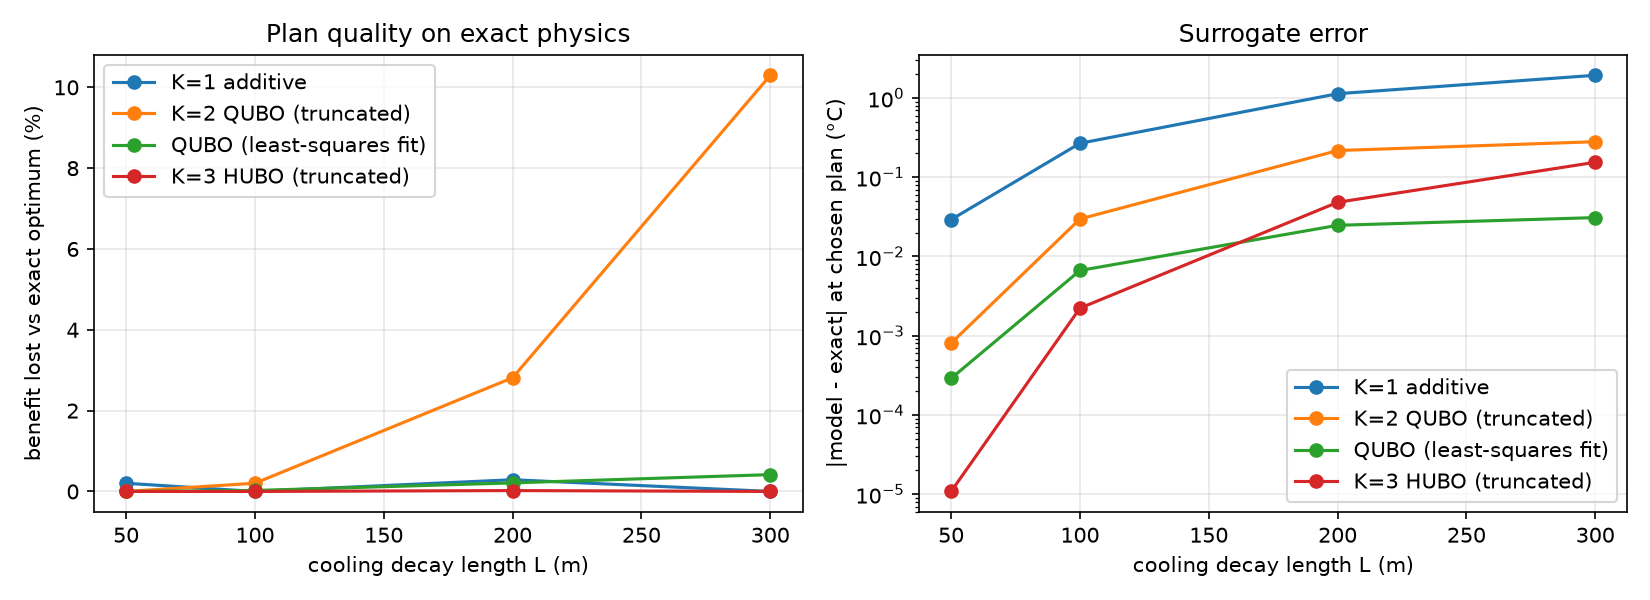
\includegraphics[width=0.8\linewidth]{e2_fidelity.png}\caption{E2 fidelity versus decay length.}\end{figure}
\paragraph{Reading.} When kernels overlap strongly, the second-order truncation over-counts
diminishing returns, believes clustered parks are much worse than they are, and spreads them out:
at $L=300$\,m the Taylor \QUBO{} loses 10.30\%. The cubic \HUBO{} loses at most 0.02\%; a \QUBO{}
with the same 253 coefficients fitted by least squares loses at most 0.42\%. The number of terms
grows from 22 ($K{=}1$) to 253 ($K{=}2$) to 1{,}793 ($K{=}3$).

\section{E4: penalty-weight sweep}
\exphead{How does the penalty weight trade feasibility against sampler quality?}
{$\Lam/\Lsafe\in\{0.01,\dots,3\}$, 3 seeds $\times$ 32 reads, mix $8\times8$ + equity and park $12\times12$.}
{\code{results/E4\_penalty/}}{E4}
\begin{table}[!htbp]\centering\caption{E4 (typed from \code{docs/RESULTS.md}).}\small% typed from docs/RESULTS.md (E4; full table: results/E4_penalty/penalty_summary.csv, appendix)
\begin{tabular}{llrrrrr}
\toprule
instance & solver & $\Lam/\Lsafe$ & P(feas) raw & \Popt{} raw & \Popt{} pp & benefit pp \\
\midrule
mix $8\times8$ + equity & SA & 0.01 & 0.10 & 0.01 & 0.42 & 0.78 \\
 & SA & 1 & 1.00 & 0 & 0.03 & 0.77 \\
 & SQA & 0.01 & 0.00 & 0 & 0.29 & 0.94 \\
 & SQA & 1 & 1.00 & 0 & 0.01 & 0.89 \\
 & Tabu & 0.01 & 0.20 & 0.01 & 0.47 & 0.83 \\
 & Tabu & 1 & 1.00 & 0 & 0 & 0.71 \\
park $12\times12$ & all & $\le0.03$ & $\le0.15$ & $\approx0$ & 1.00 & 1.00 \\
 & Tabu & $\ge0.1$ & 1.00 & 0.97--0.99 & 1.00 & 1.00 \\
\bottomrule
\end{tabular}
\end{table}
\begin{figure}[!htbp]\centering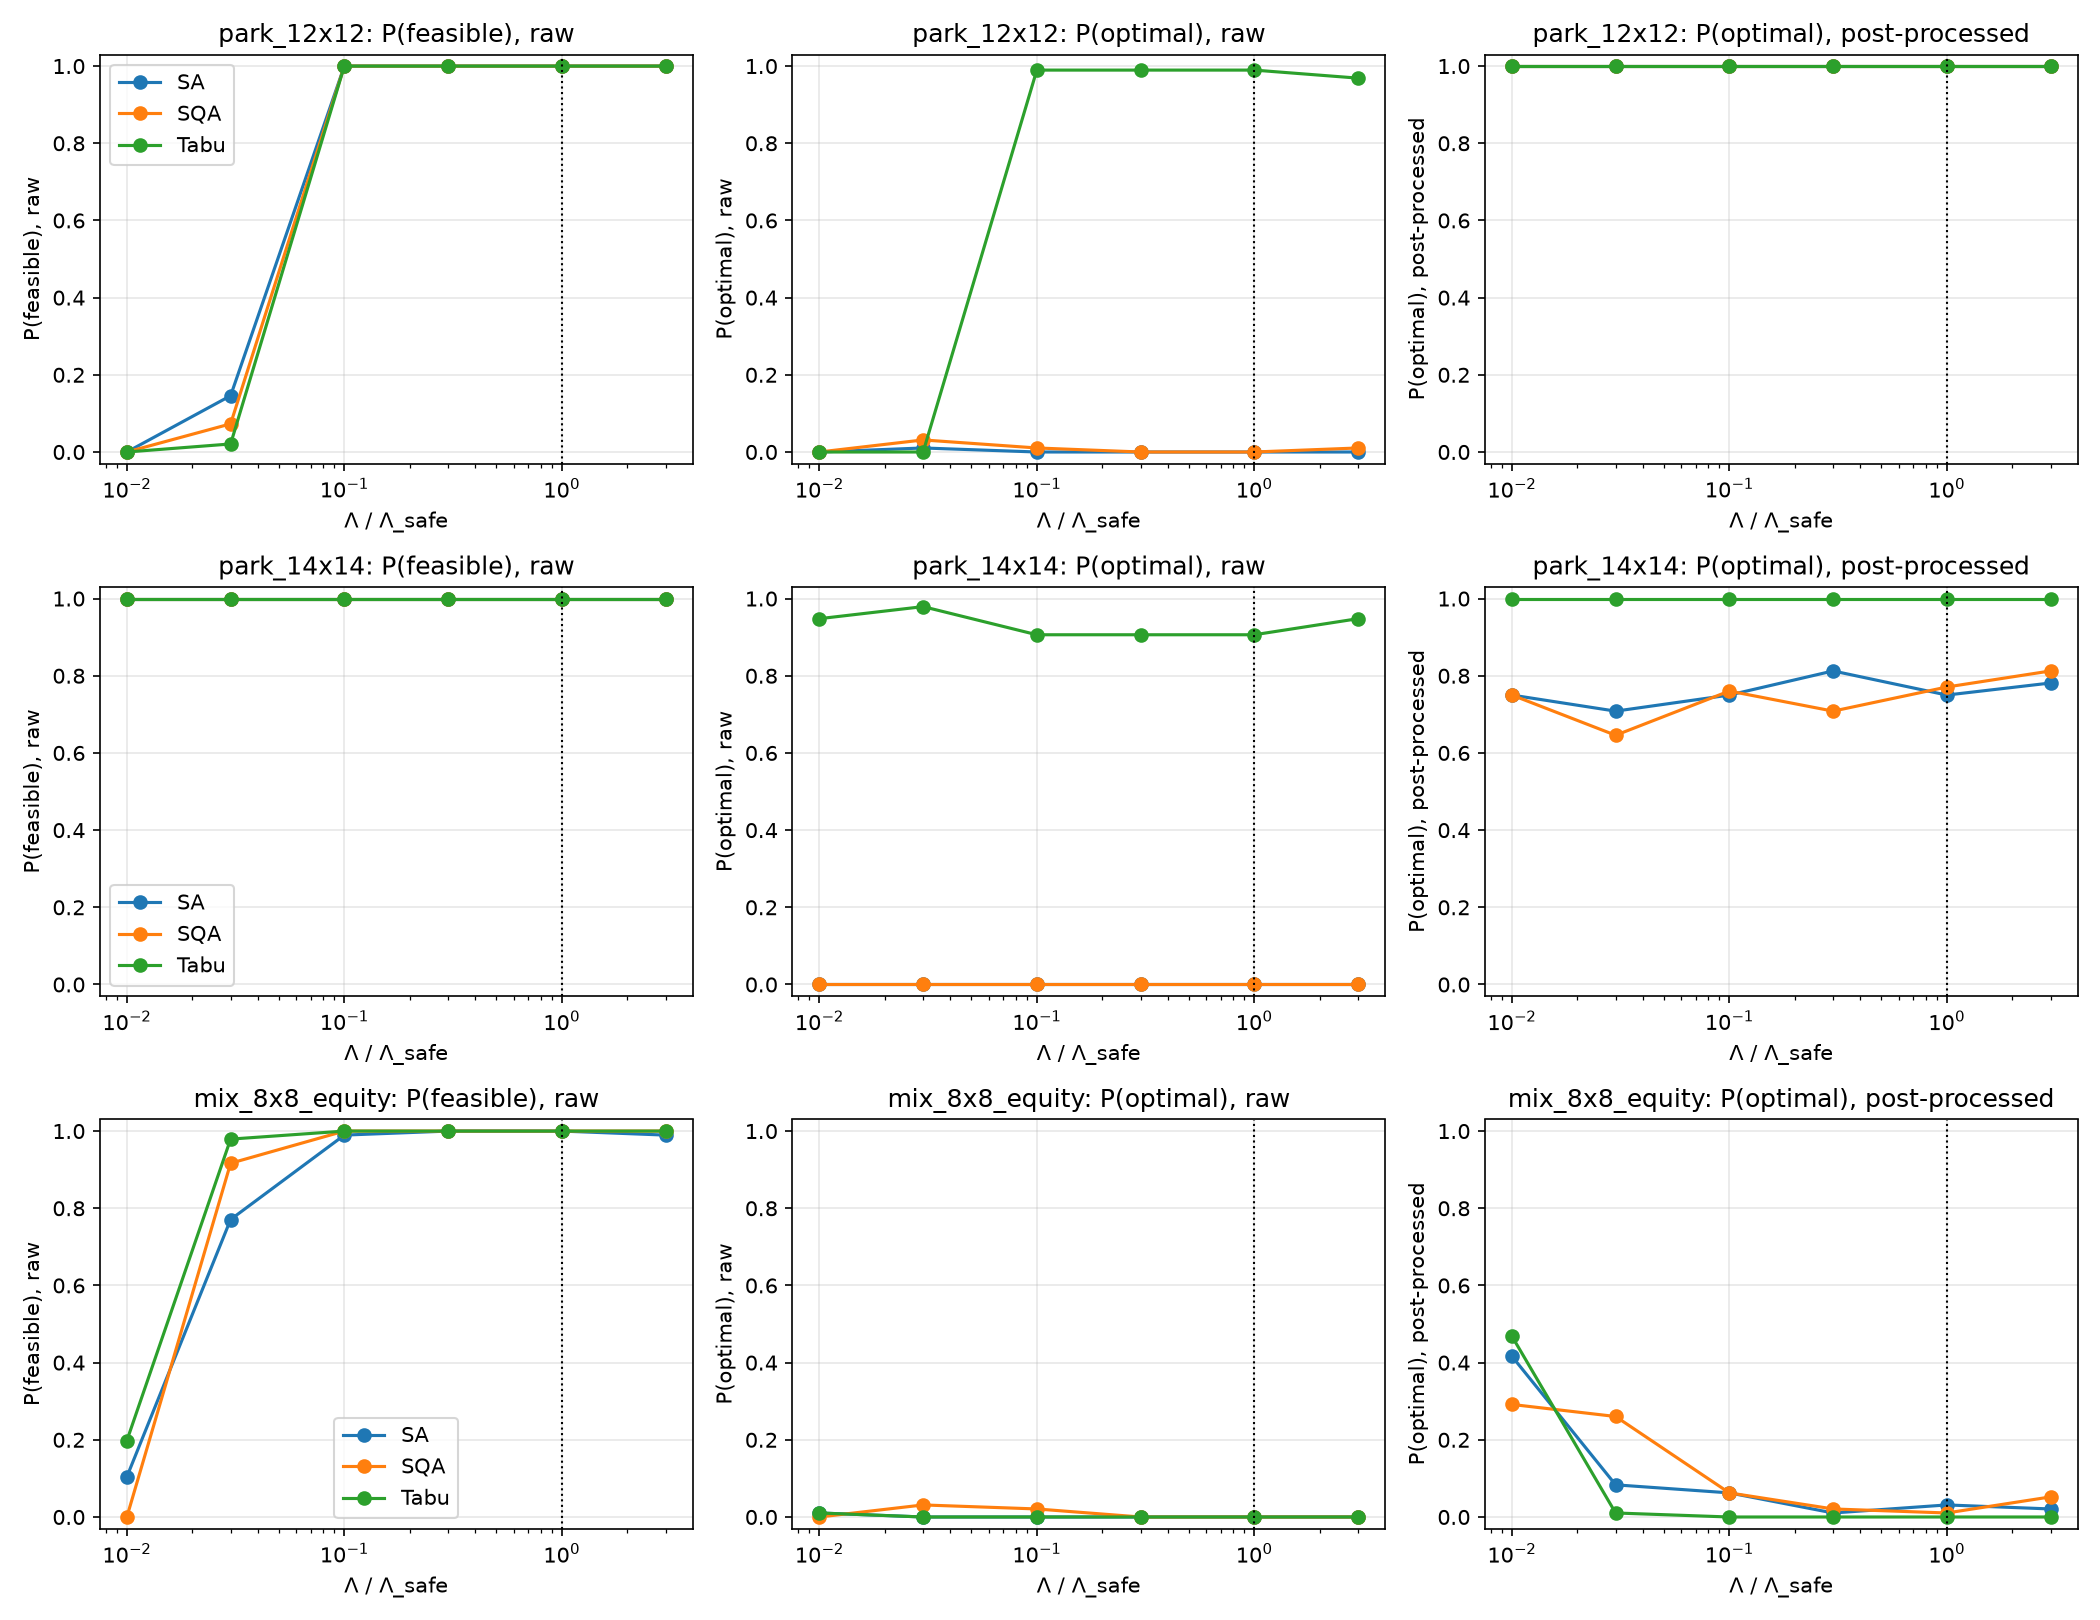
\includegraphics[width=0.6\linewidth]{e4_penalty_sweep.png}\caption{E4 penalty sweep.}\end{figure}
\paragraph{Reading.} Below about $0.1\,\Lsafe$ raw feasibility collapses, as the theory predicts,
but the infeasible low-penalty samples are better starting points for repair: $\Popt$ after
post-processing rises from at most 0.03 to 0.42 (SA) and 0.47 (Tabu). The recipe is hybrid and not
certified.

\section{E5: native HUBO versus quadratised QUBO}
\exphead{Should higher-order objectives be solved natively?}
{$10\times10$ cities, 30 decision variables, cubic saturation plus quartic park-block synergy; the
constrained \HUBO{} optimum is certified by MILP on all three instances.}{\code{results/E5\_hubo/}}{E5}
\begin{table}[!htbp]\centering\caption{E5 (generated from \code{hubo\_summary.csv}).}% generated by latex/tools/make_tables.py from results/ -- do not edit
\begin{tabular}{llrrrr}
\toprule
formulation & solver & vars & P(opt) raw & pp & benefit \\
\midrule
QUBO (Rosenberg) & Greedy & 192 & 0.000 & 1.000 & 0.849 \\
QUBO (Rosenberg) & SA & 192 & 0.000 & 1.000 & 0.837 \\
QUBO (Rosenberg) & SQA & 192 & 0.000 & 0.997 & 0.930 \\
QUBO (Rosenberg) & Tabu & 192 & 0.000 & 1.000 & 0.847 \\
native HUBO & Greedy & 30 & 0.003 & 0.976 & 0.921 \\
native HUBO & SA & 30 & 0.000 & 0.997 & 0.920 \\
native HUBO & SQA & 30 & 0.000 & 0.993 & 0.960 \\
native HUBO & Tabu & 30 & 0.990 & 1.000 & 0.999 \\
\bottomrule
\end{tabular}
\end{table}
\paragraph{Reading.} Tabu finds the optimum on 99.0\% of raw reads on the native \HUBO{} and on 0\%
after quadratisation (187--197 variables). The auxiliaries are tied to their pairs by penalties
$M>S$, creating narrow valleys that single-flip dynamics cannot cross.

\section{E10: penalty form (quick run, 2 instances)}
\exphead{Do slack-free penalties help?}{Unbalanced and linear penalties against the quadratic slack penalty; 10 vs 13 variables.}{\code{results/E10\_penalty\_form/}}{E10}
\begin{table}[!htbp]\centering\caption{E10 (generated).}\resizebox{\linewidth}{!}{% generated by latex/tools/make_tables.py from results/ -- do not edit
\begin{tabular}{llrrrrr}
\toprule
form & weight & vars & dyn.\ range & ground feas. & ground opt. & P(opt) pp \\
\midrule
quadratic slack (exact) & Λ\_safe & 13 & 163.0 & 1.000 & 1.000 & 0.719 \\
unbalanced & 0.1·Λ\_safe & 10 & 16.5 & 1.000 & 1.000 & 0.859 \\
unbalanced & 0.3·Λ\_safe & 10 & 49.0 & 1.000 & 1.000 & 0.766 \\
unbalanced & 1.0·Λ\_safe & 10 & 163.0 & 1.000 & 1.000 & 0.812 \\
linear & 0.5·μ & 10 & 0.6 & 0.000 & 0.000 & 1.000 \\
linear & 1.0·μ & 10 & 0.4 & 0.500 & 0.500 & 0.500 \\
linear & 2.0·μ & 10 & 1.0 & 1.000 & 0.000 & 1.000 \\
\bottomrule
\end{tabular}
}\end{table}
\paragraph{Reading.} The unbalanced penalty at $0.1\,\Lsafe$ cuts the dynamic range from 163 to 16.5
with an optimal ground state on these instances, but its exactness is instance-dependent. The linear
penalty is a Lagrangian relaxation: its ground states are feasible or optimal only for lucky
multipliers. This needs a full run before any claim.

\section{E11: native HUBO versus Rosenberg QUBO spectra (quick run, 2 instances)}
\exphead{Does quadratisation change the annealing bottleneck?}{Cubic ($K{=}3$) objective, 6 decision variables; exact spectra.}{\code{results/E11\_pubo\_gap/}}{E11}
\begin{table}[!htbp]\centering\caption{E11 (typed from \code{docs/RESULTS.md}).}\resizebox{\linewidth}{!}{% typed from docs/RESULTS.md (E11, quick run; source results/E11_pubo_gap/raw.csv)
\begin{tabular}{lccc}
\toprule
model & qubits & final gap & P(ground), $T{=}10$ \\
\midrule
A: native cubic \HUBO{} + slack penalty & 9 & $9.4\times10^{-5}$ / $1.1\times10^{-5}$ & $3.1\times10^{-3}$ \\
B: Rosenberg \QUBO{} of A & 16 & $9.4\times10^{-5}$ / $1.1\times10^{-5}$ & $2.4\times10^{-5}$ \\
C: native \HUBO{} on $\Fset$ (diagonal only) & 6 & $2.4\times10^{-2}$ / $3.7\times10^{-3}$ & $4.5\times10^{-2}$ / $4.1\times10^{-2}$ \\
\bottomrule
\end{tabular}
}\end{table}
\paragraph{Reading.} The final gap is set by the slack penalty and is identical to three digits for
A and B, but B needs 7 more qubits and its short-anneal ground-state probability is about
100$\times$ lower. Removing the penalty (C, diagonal-only, not hardware-realisable) enlarges the gap
about 250$\times$.

%======================================================================
\chapter{Classical bar}
\section{E3: solver scaling (certified optima, safe penalty)}
\exphead{How do penalty-\QUBO{} samplers scale against certified optima?}
{Two families, 3 instances per size $\times$ 4 seeds $\times$ 32 reads; 1{,}000 sweeps for SA/SQA,
SQA with $P=16$; SA-matched gets $(P{+}1)\times$ more sweeps; QAOA only up to 16 qubits.}
{\code{results/E3\_scaling/}}{E3}
\begin{table}[!htbp]\centering\caption{E3: median raw success per read (generated).}\resizebox{\linewidth}{!}{% generated by latex/tools/make_tables.py from results/ -- do not edit
\begin{tabular}{lrrrrrrr}
\toprule
family / vars & Greedy & SA & SA-matched & SQA & SQA-fixedT & Tabu & QAOA(p=4) \\
\midrule
park / 13 & 0.20 & 0.48 & 1.00 & 1.00 & 1.00 & 1.00 & 0.01 \\
park / 17 & 0.06 & 0.03 & 0.48 & 0.56 & 0.84 & 1.00 & -- \\
park / 27 & 0.00 & 0.00 & 0.00 & 0.00 & 0.00 & 1.00 & -- \\
park / 32 & 0.00 & 0.00 & 0.00 & 0.00 & 0.00 & 0.94 & -- \\
park / 46 & 0.00 & 0.00 & 0.00 & 0.00 & 0.00 & 0.66 & -- \\
mix+equity / 42 & 0.00 & 0.00 & 0.00 & 0.00 & 0.00 & 0.00 & -- \\
mix+equity / 56 & 0.00 & 0.00 & 0.00 & 0.00 & 0.00 & 0.00 & -- \\
mix+equity / 89 & 0.00 & 0.00 & 0.00 & 0.00 & 0.00 & 0.00 & -- \\
\bottomrule
\end{tabular}
}\end{table}
\begin{figure}[!htbp]\centering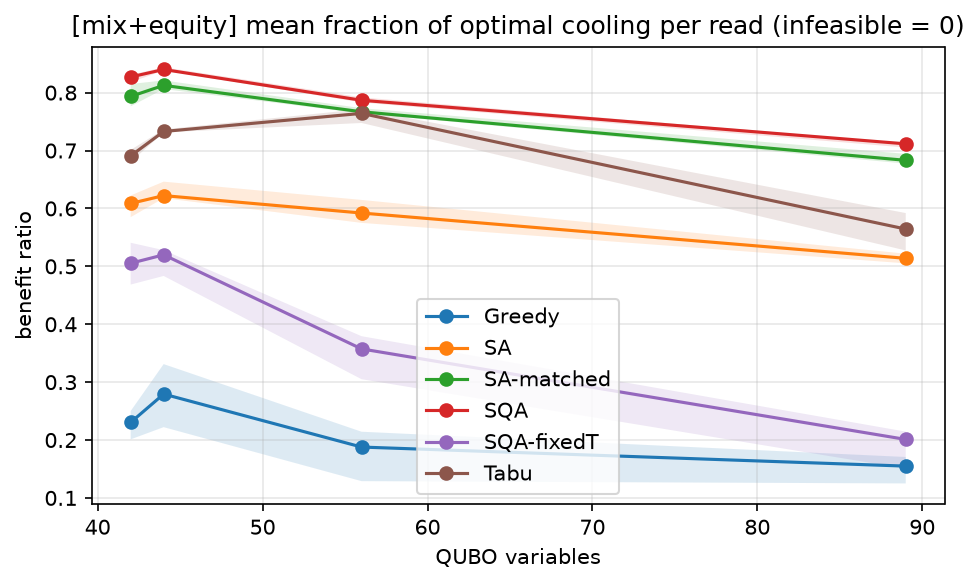
\includegraphics[width=0.7\linewidth]{e3_benefit_mix.png}\caption{E3 mean benefit per read on mix + equity.}\end{figure}
\paragraph{Reading.} Tabu is the strongest sampler on single-intervention \QUBO{}s and weaker on
the constrained multi-choice family. The SQA-over-SA advantage at equal sweeps largely disappears at
equal flips on parks (17 variables: 0.54 $\pm$ 0.07 vs 0.50 $\pm$ 0.11); on mix + equity SQA's
$+0.02$--$0.03$ benefit over SA-matched costs about 2.4$\times$ the wall time. Fixed-temperature SQA
collapses in feasibility on mix + equity. QAOA at $p=4$ on 13 qubits puts 1\% on the optimum. The
greedy planner is optimal on 8 of 15 park instances (worst gap 0.037\,\degC{}) and infeasible on 5
of 9 mix instances because it ignores equity. After post-processing, every sampler, even random,
solves most park instances, so post-processed success does not discriminate there.

\section{E7: end-to-end showcase}
\exphead{What does a full plan look like on a larger city?}
{$14\times14$ city, parks, water and cool pavement, budget 24, equity; 81 decision variables and a
105-variable \QUBO{} at $0.1\,\Lsafe$.}{\code{results/E7\_showcase/}}{E7}
\begin{table}[!htbp]\centering\caption{E7 (typed from \code{docs/RESULTS.md}).}\resizebox{\linewidth}{!}{% typed from docs/RESULTS.md (E7; source results/E7_showcase/summary.json)
\begin{tabular}{lccccc}
\toprule
plan & feasible & exposure $T$ (\degC) & pop.-weighted cooling & interventions & time \\
\midrule
baseline & -- & 32.311 & -- & 0 & -- \\
MILP (certified optimal) & yes & 31.141 & 1.231\,\degC & 8 parks & 10.8\,s \\
Greedy planner & yes & 31.141 (same plan) & 1.231\,\degC & 8 parks & $<1$\,s \\
SA + pp & yes & 31.230 & 1.140\,\degC & 10 & 12.4\,s \\
SQA + pp & yes & 31.230 (same plan as SA) & 1.140\,\degC & 10 & 32.1\,s \\
Tabu + pp & yes & 31.459 & 0.891\,\degC & 14 & 10.8\,s \\
\bottomrule
\end{tabular}
}\end{table}
\begin{figure}[!htbp]\centering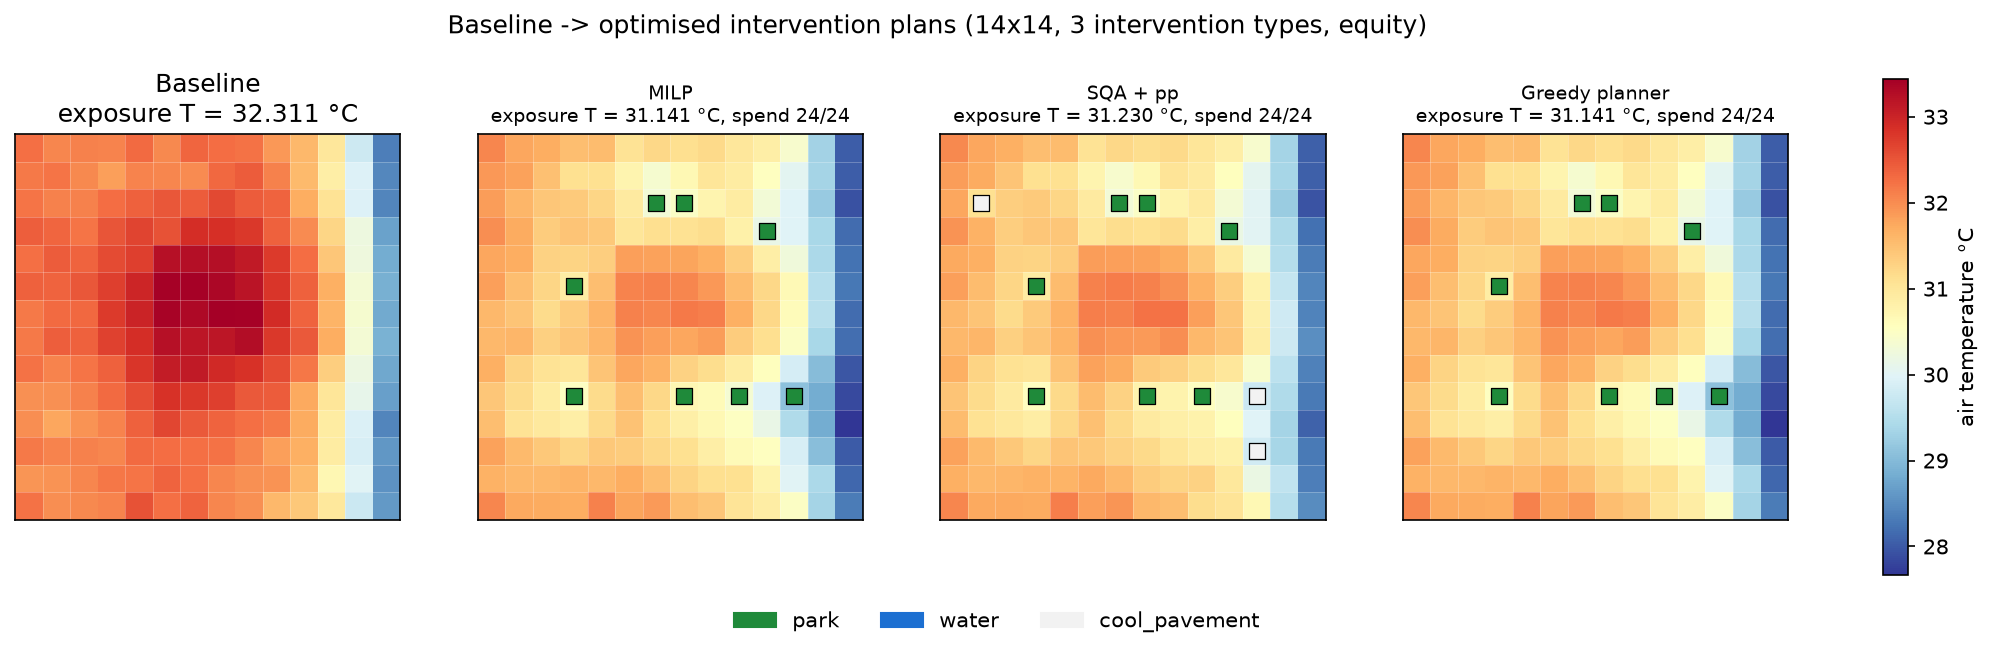
\includegraphics[width=\linewidth]{e7_transition.png}\caption{E7 baseline to optimised plans.}\end{figure}
\paragraph{Reading.} The optimal plan lowers the exposure-weighted temperature by 1.17\,\degC{};
all 20 baseline hot-spot cells drop below the hot-spot threshold under every plan. Water is never
selected (5 units for 2.0\,\degC{} is dominated by parks at 3 units for 1.5\,\degC{}). The hottest
core receives nothing because the generator places few candidate lots in dense blocks: the siting
constraint, not the optimiser, limits what can be achieved.

\section{E9: weak penalty plus repair as a declared hybrid}
\exphead{Is weak penalty + repair the best penalty-based recipe?}
{E3 mix + equity $8\times8$, $10\times10$, $12\times12$ (3 seeds each, all certified), 2 sampler
seeds, $\alpha\in\{0.01,0.03,0.1,1\}$.}{\code{results/E9\_hybrid/}}{E9}
\begin{table}[!htbp]\centering\caption{E9 (generated; full table in the appendix).}% generated by latex/tools/make_tables.py from results/ -- do not edit
\begin{tabular}{llrrrr}
\toprule
solver & $\alpha$ & P(feas) & P(opt) raw & P(opt) pp & benefit pp \\
\midrule
FeasibleSA & -- & 1.000 & 0.460 & -- & -- \\
Greedy planner & -- & 0.444 & 0.444 & -- & -- \\
MILP (HiGHS) & -- & 1.000 & 1.000 & -- & -- \\
SA & 0.01 & 0.608 & 0.017 & 0.503 & 0.941 \\
SA & 1 & 0.979 & 0.000 & 0.031 & 0.813 \\
SA-matched & 0.01 & 0.715 & 0.168 & 0.804 & 0.976 \\
SA-matched & 1 & 1.000 & 0.003 & 0.184 & 0.896 \\
SQA & 0.01 & 0.833 & 0.156 & 0.767 & 0.979 \\
SQA & 1 & 1.000 & 0.003 & 0.108 & 0.880 \\
Tabu & 0.01 & 0.792 & 0.078 & 0.321 & 0.903 \\
Tabu & 1 & 0.983 & 0.000 & 0.009 & 0.748 \\
\bottomrule
\end{tabular}
\end{table}
\paragraph{Reading.} $\alpha=0.01$ plus repair raises post-processed $\Popt$ from at most 0.18 (safe
$\Lam$) to 0.77--0.80 for SQA and SA-matched. SQA gains nothing over compute-matched SA. Greedy
violates equity on 5 of 9 instances; MILP certifies in 3.8\,s on average. Nothing here meets MILP's
$\Popt=1$.

\section{HiGHS wall-clock across studies}
\begin{center}\small
\begin{tabular}{lll}
\toprule
study & instances & HiGHS wall \\
\midrule
E7 showcase & 1 & 10.8\,s \\
E9 (mix + equity) & 9 & 3.8\,s mean \\
E12 family H & 9 & 0.81\,s mean, 2.29\,s max \\
E12b family H & 9 & 0.77\,s mean \\
E12b family C & 3 & 0.013\,s mean \\
E13 tile & 1 & 1.67\,s \\
\bottomrule
\end{tabular}
\end{center}
Certification becomes slow above about 60 dense decision variables: a $20\times20$ pilot was not
certified in 120\,s.

%======================================================================
\chapter{Quantum simulation and QAOA}
\section{E6: small-scale quantum simulation (14 qubits)}
\exphead{What limits analog annealing and QAOA on the certified penalty \QUBO{}?}
{$7\times7$ city, 10 decision + 4 slack qubits, $H(s)=-(1-s)\sum X+sH_P$ with $H_P$ normalised to
$[0,1]$; exact spectra, simulated anneals and QAOA.}{\code{results/E6\_quantum/}}{E6}
\begin{table}[!htbp]\centering\caption{E6 (typed from \code{docs/RESULTS.md}).}% typed from docs/RESULTS.md (E6; source results/E6_quantum/quantum_small.csv)
\begin{tabular}{lcccc}
\toprule
$\Lam/\Lsafe$ & ground = opt. & $\gap$ & $1/\Delta^2$ & QAOA $\Popt$, $p{=}6$ \\
\midrule
0.1 & yes & $7.1\times10^{-5}$ & $2.0\times10^{8}$ & 0.0019 \\
0.3 & yes & $2.4\times10^{-5}$ & $1.8\times10^{9}$ & 0.0018 \\
1 & yes & $7.1\times10^{-6}$ & $2.0\times10^{10}$ & 0.0017 \\
3 & yes & $2.4\times10^{-6}$ & $1.8\times10^{11}$ & 0.0017 \\
10 & yes & $7.1\times10^{-7}$ & $2.0\times10^{12}$ & 0.0017 \\
\bottomrule
\end{tabular}
\end{table}
\begin{figure}[!htbp]\centering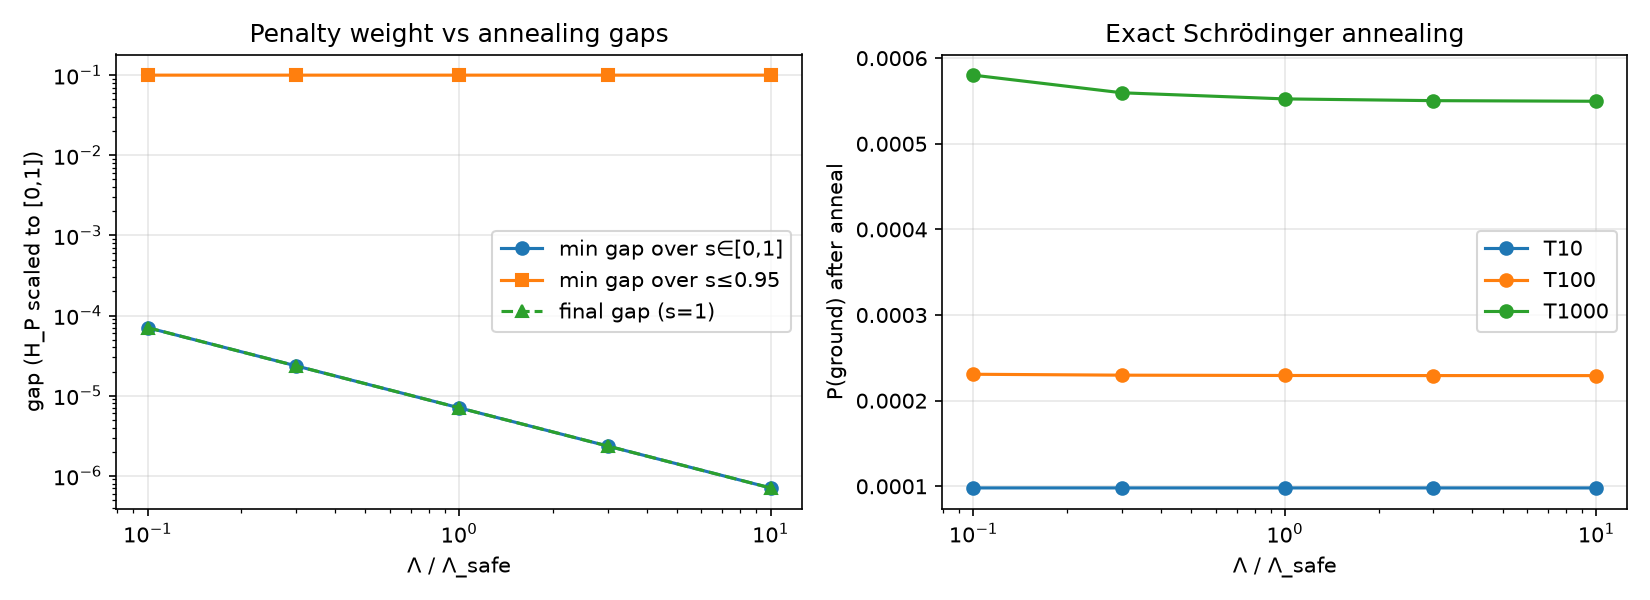
\includegraphics[width=0.8\linewidth]{e6_gap_vs_penalty.png}\caption{E6 gap versus penalty.}\end{figure}
\paragraph{Reading.} The final gap scales exactly as $1/\Lam$ and the minimum gap sits at $s=1$, so
$1/\Delta^2$ grows as $\Lam^2$, from $2\times10^{8}$ to $2\times10^{12}$. Practical anneal times
($T\le1000$) give about 9$\times$ uniform ground-state probability, independent of $\Lam$. QAOA's
approximation ratio ($\approx0.998$) is measured on a penalty-dominated scale; its optimum probability
only grows from 0.08\% ($p=1$) to 0.17--0.19\% ($p=6$), about 30$\times$ uniform
($1/2^{14}=6.1\times10^{-5}$).
\plainbox{Making the rules strict makes the energy differences between good and bad plans tiny, and
a quantum annealer would need impossibly long runs to tell them apart.}

\section{E8: constraint-preserving mixers ($p\le2$)}
\exphead{Do Dicke/XY and feasibility-projected mixers fix penalty QAOA?}
{8 park instances (including the ``exactly 3'' twin), 6 mix + equity instances with $|\Fset|$ from
720 to 2{,}243; $p\in\{1,2\}$, one L-BFGS-B run from a linear ramp plus one random restart;
heuristics 32 reads $\times$ 3 seeds.}{\code{results/E8\_mixers/}}{E8}
\begin{table}[!htbp]\centering\caption{E8 (typed from \code{docs/RESULTS.md}; full table in the appendix).}\resizebox{\linewidth}{!}{% typed from docs/RESULTS.md (E8; full table: results/E8_mixers/summary_by_family.csv, appendix)
\begin{tabular}{llrrrr}
\toprule
family & method & \Popt & P(feas) & benefit & wall (s) \\
\midrule
park & MILP & 1 & 1 & 1 & 0.09 \\
park & Greedy planner & 0.86 & 1 & 1.00 & 0.001 \\
park & XY-QAOA (swap+add/remove) $p{=}1$ / $p{=}2$ & 0.063 / 0.197 & 1 & 0.87 / 0.94 & 1.6 / 7.1 \\
park & X-mixer penalty QAOA $p{=}1$ / $p{=}2$ & 0.008 / 0.011 & 0.70 / 0.80 & 0.40 / 0.51 & 0.6 / 1.1 \\
park & FeasibleSA & 1 & 1 & 1 & 0.26 \\
park & SA / Tabu (safe-$\Lam$ QUBO) & 0.25 / 1 & 1 & 0.96 / 1 & 0.07 / 0.02 \\
exactly-3 & Dicke-XY complete $p{=}1$ / $p{=}2$ & 0.18 / 0.37 & 1 & 0.94 / 0.97 & 3 / 15 \\
exactly-3 & Dicke-XY ring $p{=}1$ / $p{=}2$ & 0.04 / 0.14 & 1 & 0.88 / 0.91 & 3 / 16 \\
exactly-3 & X-mixer penalty QAOA $p{=}1$ / $p{=}2$ & 0.004 / 0.005 & 0.45 / 0.62 & 0.35 / 0.49 & 0.2 / 0.3 \\
mix+eq & MILP & 1 & 1 & 1 & 0.18 \\
mix+eq & Greedy planner & 0.33 & 0.33 & 0.33 & 0.002 \\
mix+eq & XY-QAOA $p{=}1$ / $p{=}2$ & 0.002 / 0.003 & 1 & 0.60 / 0.61 & 3.6 / 25 \\
mix+eq & FeasibleSA & 0.39 & 1 & 0.92 & 0.79 \\
mix+eq & SA / Tabu (safe-$\Lam$ QUBO) & 0.002 / 0 & 1.0 & 0.61 / 0.61 & 0.2 / 0.14 \\
\bottomrule
\end{tabular}
}\end{table}
\paragraph{Reading.} $P(\mathrm{feasible})=1$ by construction, and $\Popt$ is 10--70$\times$ higher
than X-mixer penalty QAOA at equal depth. On mix + equity, XY-QAOA barely beats uniform sampling of
$\Fset$ ($\approx0.002$) while FeasibleSA reaches 0.39 per read. Complete-graph XY beats ring XY.
Constraint-preserving QAOA closes the gap to penalty QAOA, not to greedy or MILP.

\section{E8b: Dicke-XY depth curve}
\exphead{Is $p\le2$ simply too shallow?}
{Three ``exactly 3 parks'' $7\times7$ cities (seeds 4, 5, 6), $n=10$, $|\Fset|=120$, a single certified
optimum each; $p=1,\dots,6$; L-BFGS-B from a linear ramp plus one random restart, maxiter 300.}
{\code{results/E8b\_depth/}}{E8b}
\begin{table}[!htbp]\centering\caption{E8b (generated): mean [min--max] $\Popt$.}\resizebox{\linewidth}{!}{% generated by latex/tools/make_tables.py from results/ -- do not edit
\begin{tabular}{lrrrrr}
\toprule
method & $p{=}1$ & $p{=}2$ & $p{=}3$ & $p{=}4$ & $p{=}6$ \\
\midrule
Dicke-XY complete & 0.134 & 0.242 [0.08--0.37] & 0.309 & 0.376 & 0.427 [0.17--0.65] \\
Dicke-XY ring & 0.034 & 0.067 [0.02--0.14] & 0.057 & 0.066 & 0.111 [0.02--0.26] \\
X-mixer penalty QAOA & 0.004 & 0.005 & 0.006 & 0.008 & 0.009 \\
\bottomrule
\end{tabular}
}\\[6pt]% generated by latex/tools/make_tables.py from results/ -- do not edit
\begin{tabular}{lrrr}
\toprule
method & \Popt & benefit & wall (s) \\
\midrule
MILP (HiGHS) & 1.000 & 1.000 & 0.317 \\
Greedy planner & 0.667 & 1.000 & $8.54\times10^{-4}$ \\
uniform on F & 0.008 & 0.849 & 0.000 \\
FeasibleSA & 1.000 & 1.000 & 0.206 \\
\bottomrule
\end{tabular}
\end{table}
\begin{figure}[!htbp]\centering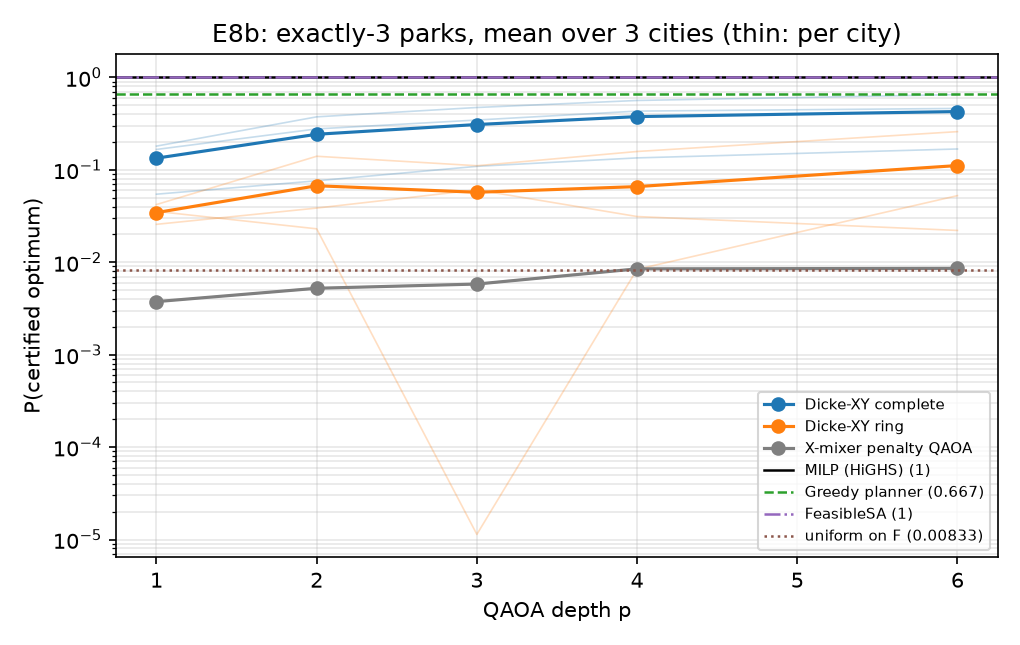
\includegraphics[width=0.6\linewidth]{p_opt_vs_p.png}\caption{E8b $\Popt$ versus depth.}\end{figure}
\paragraph{Reading.} $\Popt$ grows roughly logarithmically in $p$ (0.13 to 0.43) and is still below
0.5 at $p=6$; the worst city reaches 0.17. Ring-XY at $p=6$ (0.11) is below complete-XY at $p=1$
(0.13), and its curve is not monotone, a sign that one random restart does not reliably find the
global angles. The X-mixer puts 0.9991 of its mass on feasible strings at $p=6$ but $\Popt=0.0086$,
essentially uniform over $\Fset$: it learns the constraint, not the objective. Expected benefit for
Dicke-XY complete rises from 0.955 to 0.993. Greedy misses the surrogate optimum on one city but
scores 1.001 on the exact physics, a surrogate effect.
\specbox{ConstrainedQAOA is an exact state-vector simulation on $\mathrm{span}(\Fset)$ from a dense
$|\Fset|\times|\Fset|$ eigendecomposition. It is not a compiled gate circuit. At $p=6$ the wall-clock
(8--15\,s per city) is spent in the classical angle optimiser.}

\section{ANIM: animated comparisons}
\exphead{How does each method move in its own search space, and what does its incumbent do to the temperature field?}
{Showcase A: the E8b seed-4 ``exactly 3'' city ($n=10$). Showcase B: the E9 $10\times10$ mix +
equity city, seed 0 ($n=39$, budget 18). At most 40 frames per GIF at 10\,fps; fixed temperature
and cooling scales per instance.}{\code{results/ANIM/} (23 GIFs, \code{manifest.json})}{ANIM}
\begin{figure}[!htbp]\centering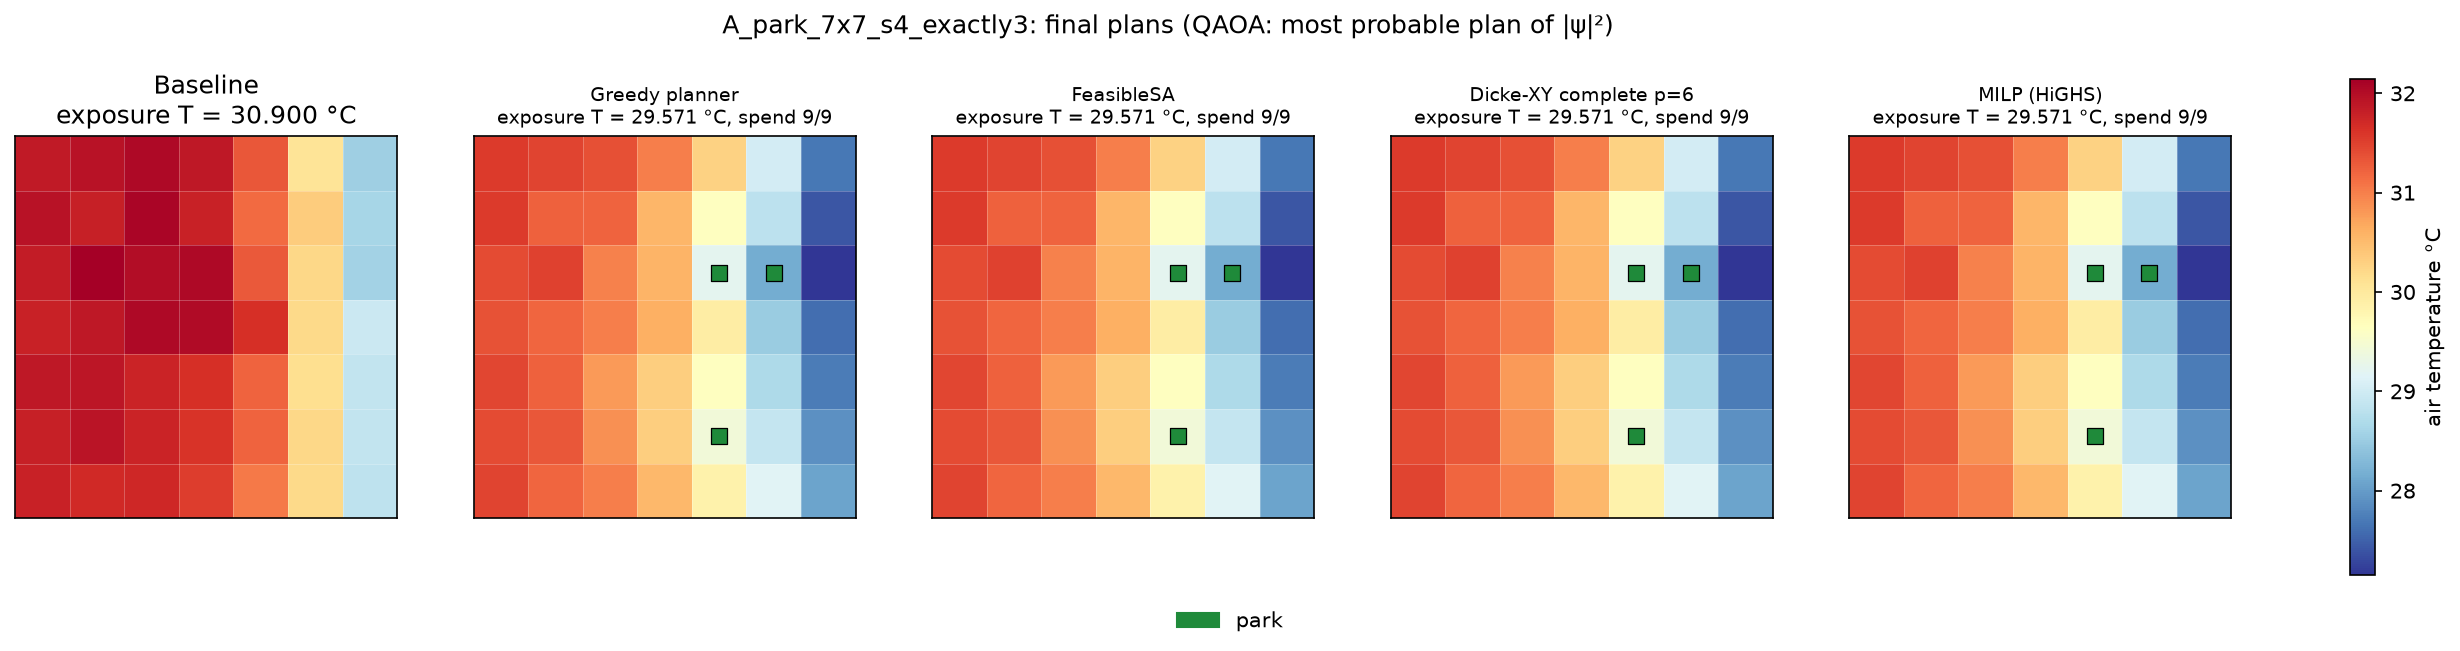
\includegraphics[width=\linewidth]{compare_final.png}\caption{Showcase A, final plans: greedy, FeasibleSA, Dicke-XY $p=6$ (most probable plan), MILP.}\end{figure}
\begin{figure}[!htbp]\centering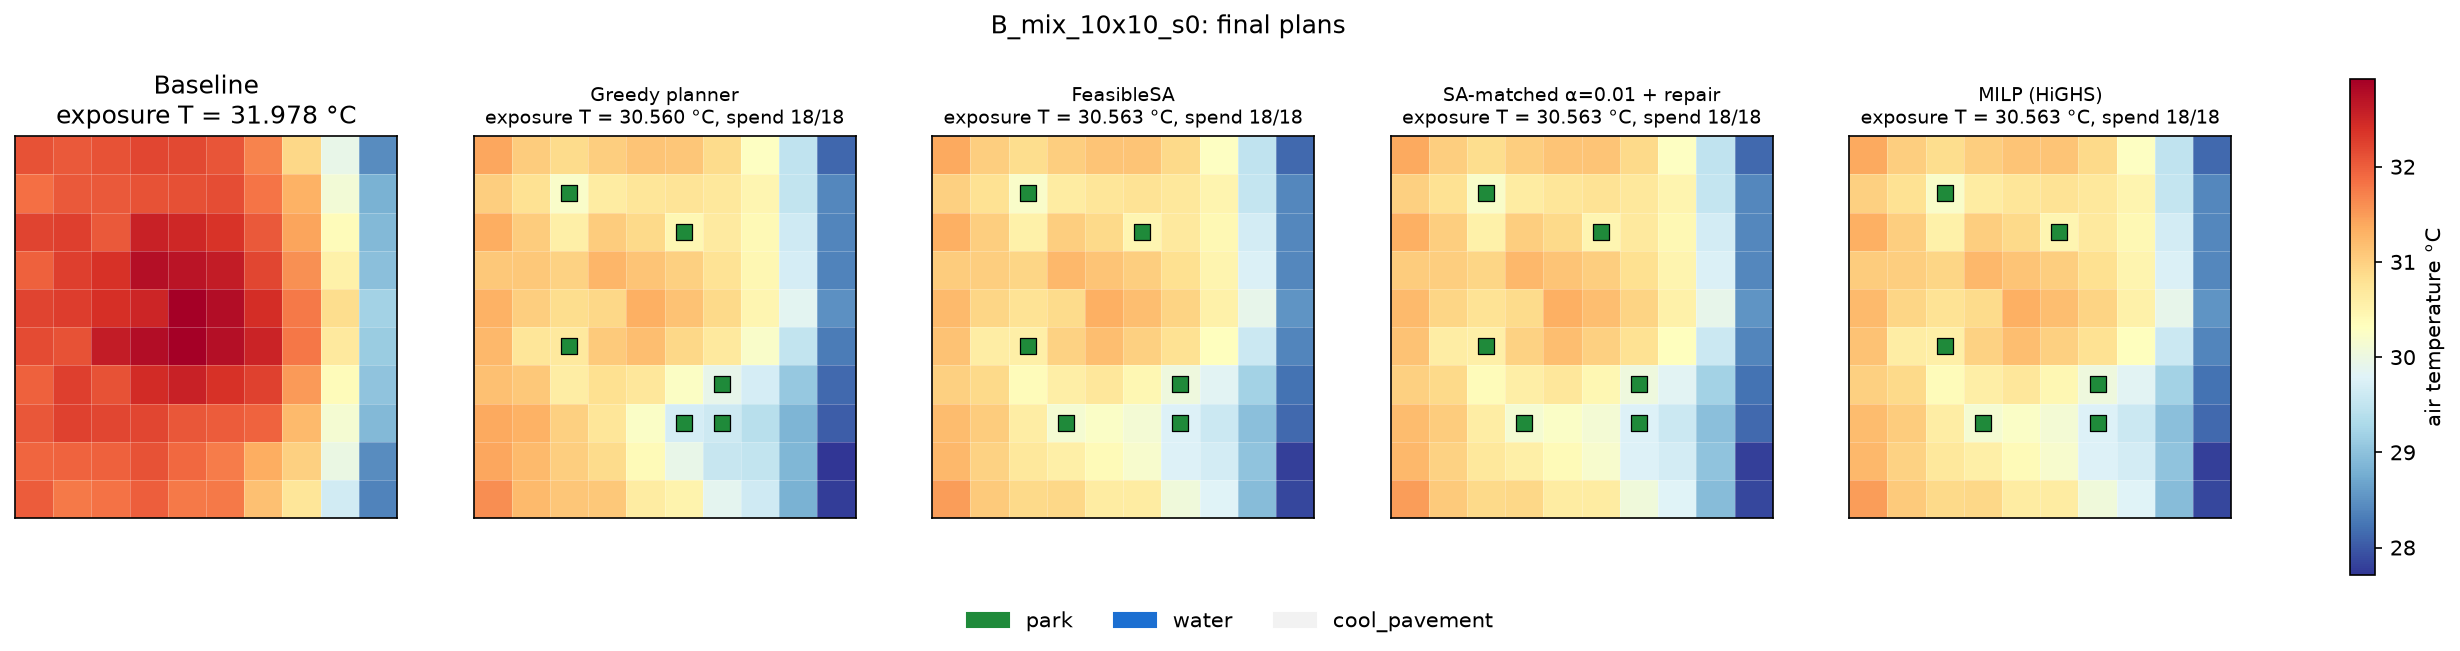
\includegraphics[width=\linewidth]{compare_final_B.png}\caption{Showcase B, final plans: greedy (infeasible on equity), FeasibleSA, weak-penalty hybrid (in place of QAOA, $|\Fset|>4000$), MILP.}\end{figure}
\paragraph{Reading.} In showcase A all four columns end on the same plan ($T=29.571$\,\degC{}); the
QAOA column keeps flickering because its draws miss the optimum 35\% of the time. In showcase B the
greedy column ends infeasible. GIFs are not embedded; they are linked:
\begin{itemize}\scriptsize\sloppy
\item \blob{results/ANIM/compare_temp_A_park_7x7_s4_exactly3.gif}
\item \blob{results/ANIM/compare_temp_B_mix_10x10_s0.gif}
\item \blob{results/ANIM/search_dicke_xy_complete_p6_A_park_7x7_s4_exactly3.gif}
\item \blob{results/ANIM/search_xmixer_penalty_qaoa_p6_A_park_7x7_s4_exactly3.gif}
\end{itemize}
\specbox{Each method lives in a different space. QAOA GIFs show $|\psi|^2$ over $\Fset$ (or over
all $2^{10}$ strings for the X-mixer); SA, Tabu and SQA show $f+\Lam P$ on the penalty \QUBO{};
FeasibleSA shows constrained $f(x)$. The two energy axes are not comparable. Every map is computed
from a real plan.}

%======================================================================
\chapter{Feasible-space PIMC: E12 and E12b}
\section{FeasibleSQA}
\paragraph{FeasibleSQA.} Path-integral Monte Carlo~\cite{martonak2002} with $P=8$ Trotter slices,
each a feasible plan, samples
$\pi(X)\propto\exp\bigl(-\tfrac{\beta}{P}\sum_k f(x^k)+J\sum_{k,i}s^k_is^{k+1}_i\bigr)$ with
$J=\tfrac12\ln\coth(\beta\Gamma/P)$, using the FeasibleSA moves on one slice at a time. It
reproduces the exact single-qubit $\langle\sigma_z\rangle$ and is quantum-\emph{inspired}: no
annealer implements a transverse field restricted to $\Fset$~\cite{heim2015}.

\paragraph{E12: matched wall-clock.} Family H has 9 instances ($8\times8$, $10\times10$,
$12\times12$ cities, seeds 100--102) with three intervention types, budget equal to the grid side,
equity, and a quartic synergy on the two larger sizes. Each method gets $\Tstar$ per run, the
larger of default FeasibleSA's median wall-clock and HiGHS's (capped at 8\,s). The pre-committed
COMPARABLE rule requires $P(\mathrm{feas})=1$, a family-mean benefit of at least 0.95$\times$ the
best classical mean, and no run over $1.5\,\Tstar$. FeasibleSQA passes with 0.981
(Table~\ref{tab:e12}), but FeasibleSA (0.973) and Tabu-on-F (0.976) pass the same bar, MILP reaches
1.000 in 0.81\,s, and the QAOA contestants do not qualify.

\paragraph{E12b: the ablation.} HiGHS was faster than default FeasibleSA on every instance, so
E12's $\Tstar$ was FeasibleSA's own time and there was no padding. The difference was work:
FeasibleSQA rejects moves that would leave $\Fset$ before evaluating $f$, so in the same wall-clock
it made 3.6$\times$ as many proposals (4.66\,M against 1.30\,M per run). Giving every method the
same proposal budget $\Wstar$ (4.53\,M per run on average) reverses the order: FeasibleSA 0.988,
FeasibleSQA 0.983, Tabu-on-F 0.977 (Table~\ref{tab:e12b}). FeasibleSQA stays within 5\% of
FeasibleSA (it is ahead on 1 instance, tied on 6, behind on 2) but does not beat it. E12 must not be
cited as a quantum-inspired win.


\section{E12: comparable-performance bakeoff}
\exphead{At matched wall-clock, does any quantum or quantum-inspired method reach 0.95 of the best classical benefit on a hard family?}
{Family H (9 instances) and family C (3), two sampler seeds; $\Tstar$ as defined above; contestants
FeasibleSQA ($P=8$, 500 sweeps, 2 reads per batch), QAOA-seeded FeasibleSA and ConstrainedQAOA
$p=2,4$ (only if $|\Fset|\le4000$), X-mixer penalty QAOA (negative control, $\le14$ qubits). The
definition was committed before the run.}{\code{results/E12\_comparable/}}{E12}
\begin{table}[!htbp]\centering\caption{E12 family H (generated; family C in the appendix).}\label{tab:e12}% generated by latex/tools/make_tables.py from results/ -- do not edit
\begin{tabular}{lrrrrrc}
\toprule
method (family H) & P(feas) & \Popt & benefit & min & wall (s) & comp. \\
\midrule
MILP (HiGHS, 8 s cap) & 1.000 & 1.000 & 1.000 & 1.000 & 0.809 & yes \\
Greedy planner & 0.333 & 0.333 & 0.333 & 0.000 & 0.009 & no \\
FeasibleSA & 1.000 & 0.778 & 0.973 & 0.813 & 7.693 & yes \\
Tabu-on-F & 1.000 & 0.778 & 0.976 & 0.708 & 8.120 & yes \\
SA-matched α=0.01 + repair & 0.833 & 0.722 & 0.831 & 0.000 & 7.847 & no \\
FeasibleSQA & 1.000 & 0.722 & 0.981 & 0.854 & 7.975 & yes \\
QAOA-seeded FeasibleSA & 1.000 & 0.833 & 0.873 & 0.000 & 8.095 & no \\
ConstrainedQAOA p=2 & 1.000 & 0.500 & 0.658 & 0.000 & 2.008 & no \\
ConstrainedQAOA p=4 & 1.000 & 0.167 & 0.665 & 0.000 & 2.221 & no \\
\bottomrule
\end{tabular}
\end{table}
\begin{figure}[!htbp]\centering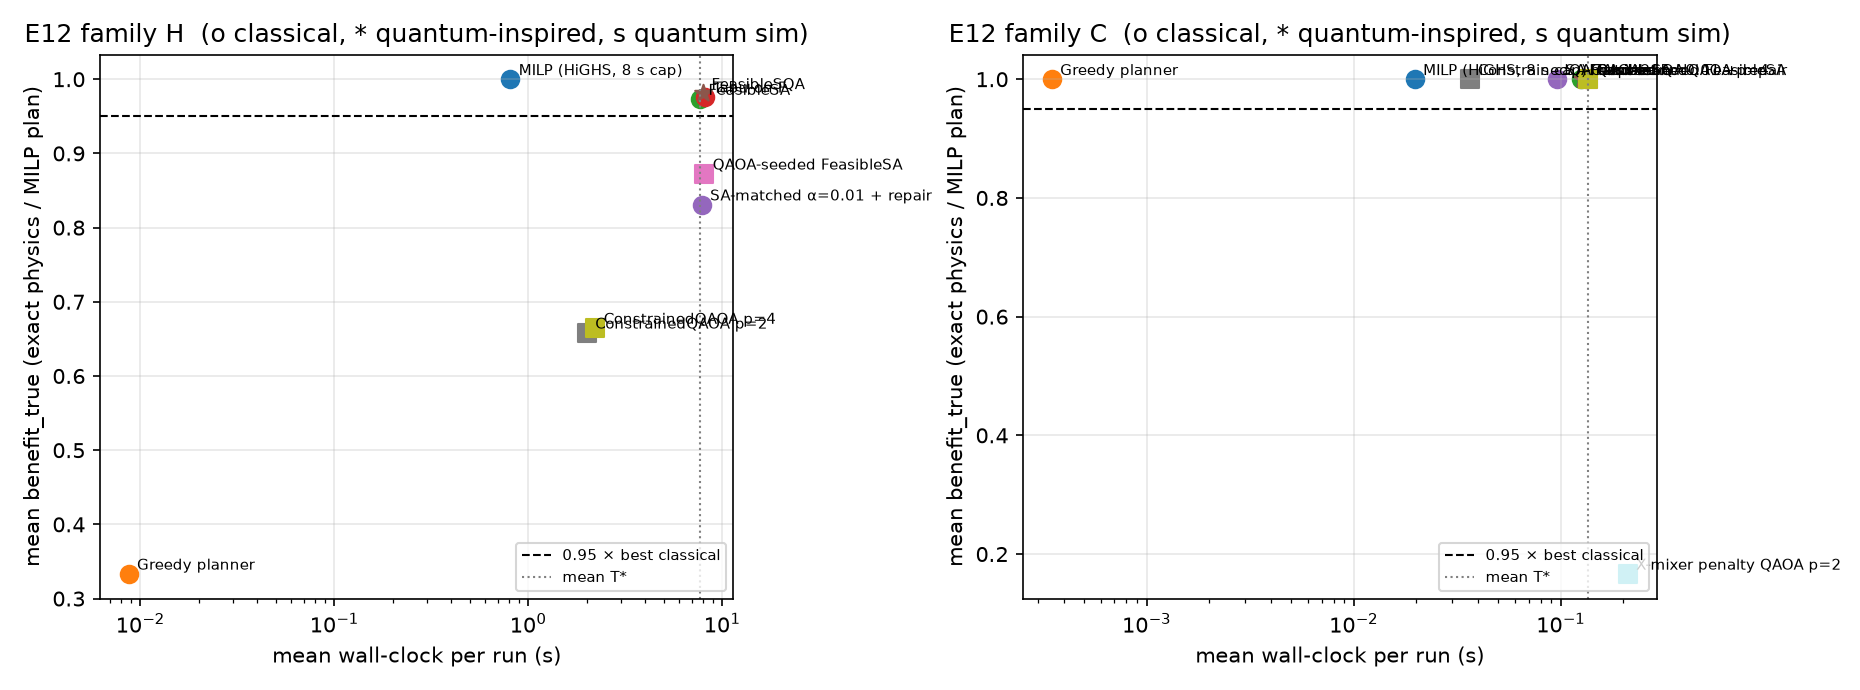
\includegraphics[width=\linewidth]{e12_benefit_vs_time.png}\caption{E12 benefit versus wall-clock, families H and C.}\end{figure}
\paragraph{Reading.} $\Tstar$ is 1.4--1.6\,s on $8\times8$, 4.0--4.7\,s on $10\times10$ and
18--20\,s on $12\times12$ (0.13--0.15\,s on C). MILP certifies all 12 instances. FeasibleSQA is
COMPARABLE by the pre-committed rule (0.981, minimum 0.85), and so are FeasibleSA (0.973) and
Tabu-on-F (0.976); the whole difference comes from the $12\times12$ synergy cities and is within
seed noise. ConstrainedQAOA is only simulable on $8\times8$; on the $|\Fset|=2484$ city the
subspace setup exceeds $\Tstar$ and scores 0. The E9 hybrid is best on $10\times10$ and
$12\times12$ but fails on all three $8\times8$ cities because greedy repair cannot restore
feasibility when the budget is tight and equity binds. On family C every method except the X-mixer
control reaches 1.000.

\section{E12b: equal-work and tight-clock ablation}
\exphead{After removing any padding and equalising proposals, does FeasibleSQA still match FeasibleSA?}
{Same instances and configurations. Tight clock: FeasibleSA's median E12 wall-clock per instance.
Equal work: $\Wstar$ = proposals FeasibleSQA used in E12 (median batches $\times$ 2 reads $\times$
500 sweeps $\times$ 8 slices $\times\,n$), 2.1--8.2\,M on H and 0.3--0.5\,M on C, given to every
method.}{\code{results/E12b\_ablation/}}{E12b}
\begin{table}[!htbp]\centering\caption{E12b family H, both clocks (generated).}\label{tab:e12b}\resizebox{\linewidth}{!}{% generated by latex/tools/make_tables.py from results/ -- do not edit
\begin{tabular}{llrrrrrccc}
\toprule
method & clock & \Popt & benefit & min & wall (s) & prop.\ (M) & $\geq$0.95 FSA & beats & w/t/l \\
\midrule
MILP (HiGHS, 8 s cap) & none & 1.000 & 1.000 & 1.000 & 0.77 & -- & -- & -- & -- \\
FeasibleSA & tight & 0.778 & 0.973 & 0.813 & 7.13 & 1.30 & yes & no & -- \\
Tabu-on-F & tight & 0.833 & 0.977 & 0.708 & 7.45 & 2.96 & yes & yes & 2/5/2 \\
FeasibleSQA & tight & 0.722 & 0.981 & 0.854 & 7.42 & 4.66 & yes & yes & 3/6/0 \\
QAOA-seeded FeasibleSA & tight & 1.000 & 0.667 & 0.000 & 2.07 & 0.18 & no & no & 0/2/1 \\
FeasibleSA & equal\_work & 0.889 & 0.988 & 0.854 & 24.99 & 4.53 & yes & no & -- \\
Tabu-on-F & equal\_work & 0.833 & 0.977 & 0.708 & 11.32 & 4.65 & yes & no & 1/6/2 \\
FeasibleSQA & equal\_work & 0.778 & 0.983 & 0.813 & 7.09 & 4.53 & yes & no & 1/6/2 \\
QAOA-seeded FeasibleSA & equal\_work & 1.000 & 1.000 & 1.000 & 2.28 & 2.20 & yes & no & 0/3/0 \\
\bottomrule
\end{tabular}
}\end{table}
\paragraph{Reading.} The tight clock reproduces E12 (FeasibleSQA 0.981, FeasibleSA 0.973) because
HiGHS never set $\Tstar$. In that time FeasibleSQA made 3.6$\times$ as many proposals (4.66\,M vs
1.30\,M). At equal proposals FeasibleSA reaches 0.988 and FeasibleSQA 0.983 (w/t/l 1/6/2): within
5\% (threshold 0.938), not ahead. FeasibleSQA needs less wall-clock per proposal (7.1\,s vs 25\,s),
an implementation property of early rejection. Tabu-on-F does not improve with more work (0.977).
QAOA-seeded FeasibleSA reaches 1.000 on the three $8\times8$ cities with QAOA time excluded, as does
FeasibleSA. Family C: every method reaches 1.000 on both clocks.

\textbf{Erratum.} E12's FeasibleSQA benefit of 0.981 used 3.6$\times$ the proposals of FeasibleSA.
At equal proposals FeasibleSQA scores 0.983, below FeasibleSA's 0.988. E12 must not be cited as a
quantum-inspired win.
\plainbox{The quantum-inspired method looked slightly better only because it tried more candidate
plans in the same time. Given the same number of tries, the ordinary method is slightly better.}

%======================================================================
\chapter{E13: an LST-shaped tile}
\exphead{Does a land-surface-temperature-shaped tile with scarce core lots open a classical gap?}
{One $16\times16$ city, seed 0: compact hot core (+6\,\degC{}) and cool edge ($-1.5$\,\degC{}),
population on the core, candidate lots removed from the core except 2; DEFAULT\_MIX, equity, budget
16, 0.3\,\degC{} synergy; $n=108$, $|\Fset|>4000$; tight clock 68.59\,s; two sampler seeds.}
{\code{results/E13\_tile/}}{E13}
\begin{table}[!htbp]\centering\caption{E13 (typed from \code{results/E13\_tile/e13.md}).}\label{tab:e13}% generated by latex/tools/make_tables.py from results/ -- do not edit
\begin{tabular}{lrrrr}
\toprule
method & P(feas) & \Popt & benefit & wall (s) \\
\midrule
MILP (HiGHS, 8 s cap) & 1.0 & 1.0 & 1.0000 & 1.67 \\
Greedy planner & 0.0 & 0.0 & 0.0000 & 0.06 \\
FeasibleSA & 1.0 & 0.5 & 0.9569 & 66.56 \\
Tabu-on-F & 1.0 & 0.0 & 0.6412 & 67.35 \\
FeasibleSQA & 1.0 & 0.5 & 0.9998 & 63.72 \\
SA-matched α=0.01 + repair & 1.0 & 1.0 & 1.0000 & 64.68 \\
\bottomrule
\end{tabular}
\end{table}
\begin{figure}[!htbp]\centering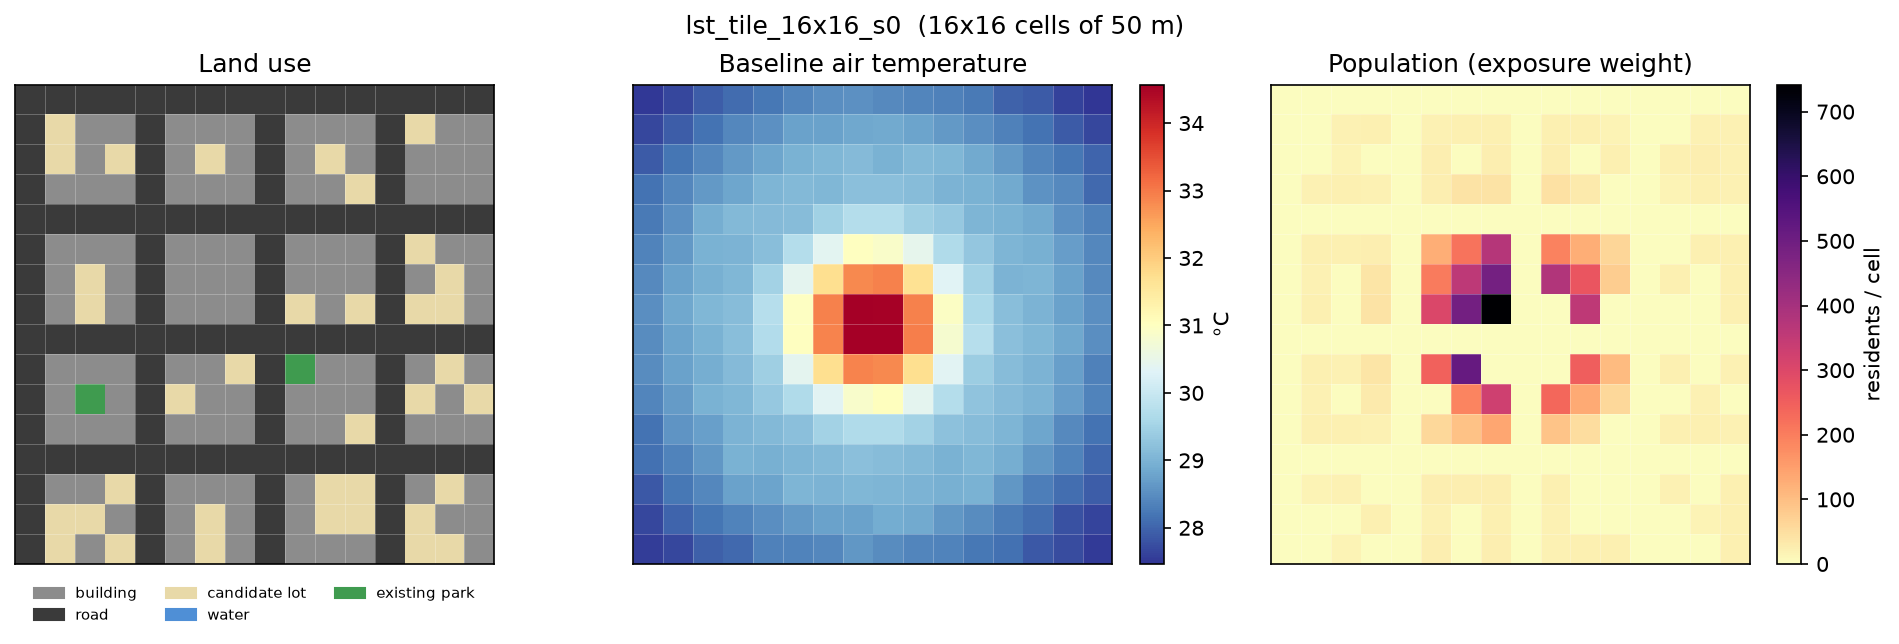
\includegraphics[width=\linewidth]{e13_city.png}\caption{E13 tile: land use, baseline temperature, population.}\end{figure}
\begin{figure}[!htbp]\centering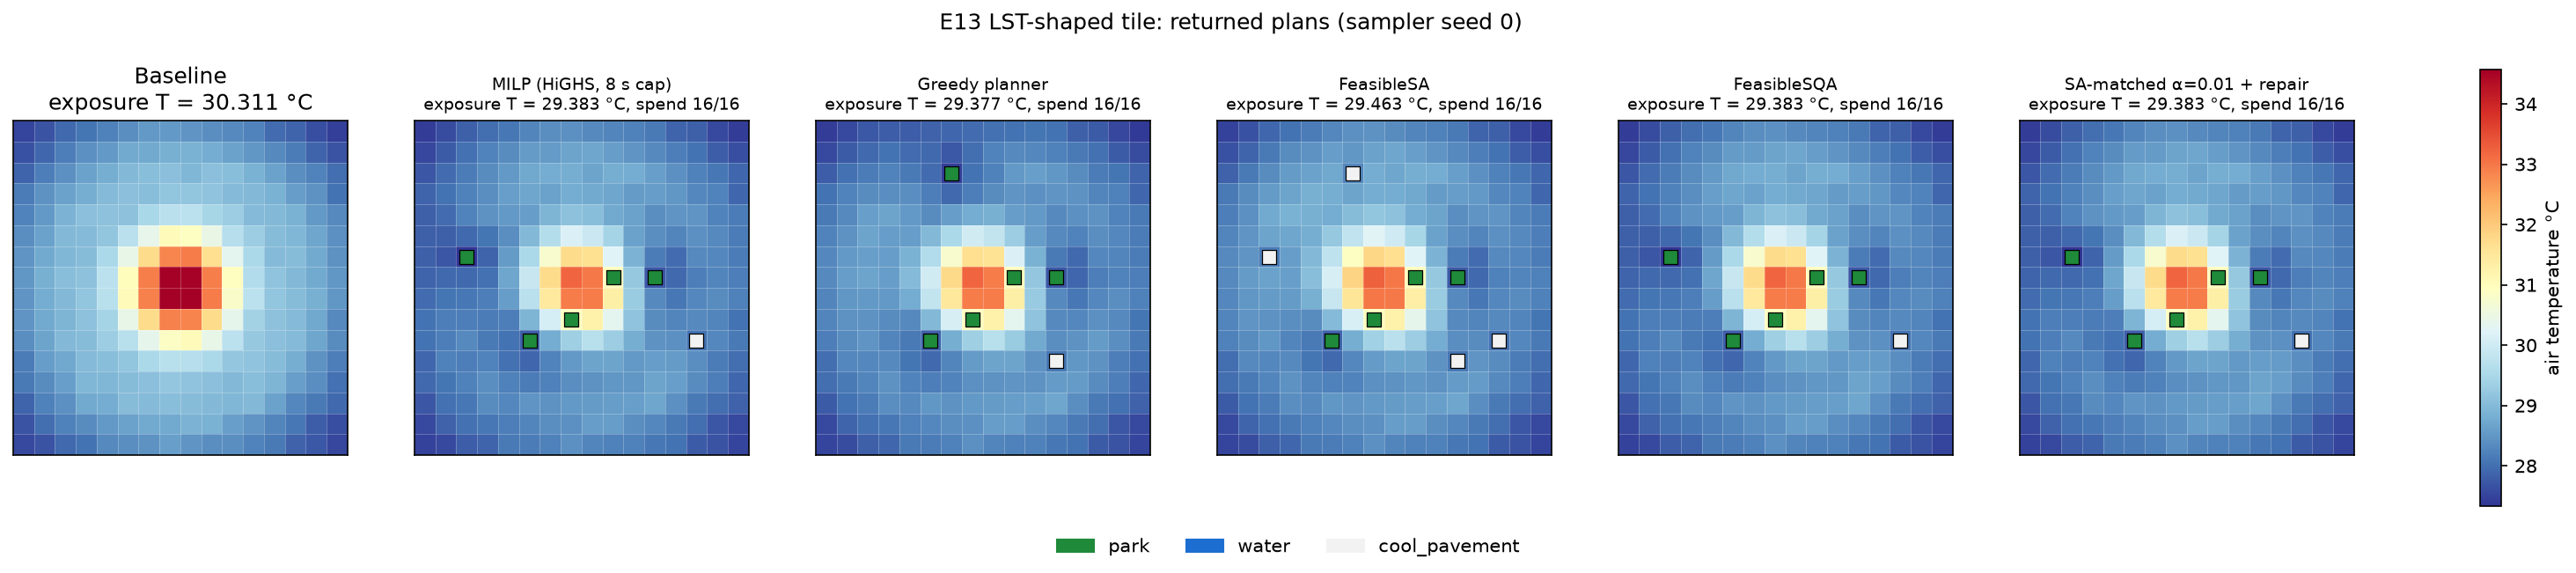
\includegraphics[width=\linewidth]{e13_plans.png}\caption{E13 returned plans (sampler seed 0).}\end{figure}
\paragraph{Reading.} E13 builds one land-surface-temperature-shaped $16\times16$ tile: a compact hot core with a cool
edge, population concentrated on the core, and only 2 candidate lots left inside the core. With
three intervention types, equity and a budget of 16 it has $n=108$ and $|\Fset|>4000$, so
ConstrainedQAOA cannot be simulated. At a tight clock of 68.59\,s per run (Table~\ref{tab:e13}),
HiGHS certifies the tile in 1.67\,s and the greedy planner is infeasible on equity, the same failure
as on family H. The weak-penalty hybrid ($0.01\,\Lsafe$ + repair) finds the optimum on both seeds,
FeasibleSQA averages 0.9998 and FeasibleSA 0.9569 on two seeds each; by E12b a tight-clock
comparison hands FeasibleSQA several times more proposals, so this gap is not evidence of an
advantage. The mask created no classical gap.


%======================================================================
\chapter{Synthesis}
\section{Hold-ups}\label{sec:holdups}
The obstacles to a quantum or quantum-inspired result, each with the experiment that shows it:
\begin{enumerate}
\item \textbf{Encoding.} Slack penalties compress the objective against the spectrum width; the final
gap scales as $1/\Lam$ (E6) and is unchanged by quadratisation (E11).
\item \textbf{Rosenberg quadratisation.} 6.4$\times$ as many variables and deep narrow valleys; Tabu
drops from 99.0\% to 0\% (E5).
\item \textbf{SA matching.} SQA's advantage at equal sweeps disappears at equal flips (E3), SQA gains
nothing over compute-matched SA in the hybrid (E9), and FeasibleSQA's lead disappears at equal
proposals (E12b).
\item \textbf{Submodularity.} Without equity, $-f$ is monotone submodular and greedy is optimal on 8 of
15 park instances (E3) and on the E7 showcase.
\item \textbf{Mixers.} Constraint-preserving mixers fix feasibility, not optimality: $\Popt=0.43$ at
$p=6$ (E8b), 0.003 at $p=2$ on mix + equity (E8).
\item \textbf{Cosmetic approximation ratios.} QAOA ratios near 0.998 on penalty-dominated scales hide
optimum probabilities of 0.17--0.19\% (E6).
\item \textbf{No QPU.} No constrained model was run on hardware or a hybrid cloud solver; the
repository hook is inactive without a token.
\end{enumerate}

\section{Discussion}
\paragraph{Success criterion.} The criterion of Section~\ref{sec:intro} is not met by gate-model
QAOA: with penalties it learns the constraint rather than the objective (E6, E8b), and with
constraint-preserving mixers it remains well below FeasibleSA and MILP at every depth we simulated
(E8, E8b, E12). Feasible-space PIMC meets a 0.95 bar relative to the best classical method, but it
only ties feasible-space SA, and at equal proposals it is slightly behind (E12b).

\paragraph{What decided the outcome.} Each step that improved a quantum or quantum-inspired method
was a change of \emph{encoding}: certified but gentler penalties (E1, E4, E10), native higher-order
terms instead of quadratisation (E5, E11), and moves or mixers that respect the constraints (E8,
E12). Each of those changes helped the classical methods at least as much. The objective's
submodularity makes greedy strong wherever equity does not bind, and HiGHS certifies every
benchmark instance quickly.

\paragraph{What hardware could still test.} A fair hardware test would submit the constrained
model natively, as a CQM to a hybrid solver, on the E8b ``exactly 3'' city (seed 4) and a family-C
park city (seed 100). A safe-$\Lam$ slack \QUBO{} should never be sent to a QPU, because its gap is
set by $\Lam$ (E6, E11). The repository contains a hook that is inactive without an API token; no
D-Wave result exists.

\section{Limitations}
\begin{itemize}
\item \textbf{Synthetic cities.} All cities and the E13 tile are synthetic; no Landsat LST or census
layers were used, and intervention amplitudes and decay lengths are illustrative.
\item \textbf{Surrogate physics.} The saturation law stands in for CFD or ENVI-met; MILP certifies the
$K{=}2$ surrogate, not the exact physics.
\item \textbf{PIMC $\neq$ QPU.} SQA and FeasibleSQA are classical Monte Carlo samplers~\cite{heim2015}.
\item \textbf{Simulated circuits.} ConstrainedQAOA is a subspace simulation on $\mathrm{span}(\Fset)$,
not a compiled circuit, and X-mixer QAOA is limited to $\le16$ qubits.
\item \textbf{No hardware numbers.} No D-Wave, Leap or other cloud result is reported.
\item \textbf{Small samples.} Three instances $\times$ two seeds per E12/E12b cell; E10 and E11 are quick
runs on two instances.
\end{itemize}


%======================================================================
\chapter{Reference material}
\section{Reproducibility}
All numbers come from seeded runs of
\begin{center}\code{python scripts/run\_experiments.py --only E$k$}\quad ($k\in\{$1,\dots,13, 8b, 12b, ANIM$\}$)\end{center}
and the audit from \code{python scripts/audit\_legacy.py}. The environment is recorded in
\code{results/env.json}: Python 3.11.15, numpy 2.4.6, scipy 1.17.1 (HiGHS), numba 0.67.0, Linux
x86\_64, all solvers single-threaded on a 4-core container. E10 and E11 are quick runs. The tables
in this document are regenerated with \code{python latex/tools/make\_tables.py} and the PDFs with
\code{make -C latex all}.

\section{Glossary}
\begin{description}
\item[QUBO] quadratic unconstrained binary optimisation
\item[HUBO] higher-order unconstrained binary optimisation (degree $>2$)
\item[MILP] mixed-integer linear program (solved with HiGHS)
\item[SA] simulated annealing; \emph{FeasibleSA}: Metropolis on feasible plans only
\item[SQA / PIMC] simulated quantum annealing by path-integral Monte Carlo
\item[FeasibleSQA] PIMC whose Trotter slices are all feasible plans
\item[QAOA] quantum approximate optimisation algorithm; \emph{ConstrainedQAOA}: Dicke/XY mixers simulated on $\mathrm{span}(\Fset)$
\item[CQM] constrained quadratic model (D-Wave Leap hybrid input format)
\item[LST] land surface temperature
\item[UHI] urban heat island
\end{description}

\begin{description}
\item[$\btrue$] exact-physics cooling of a plan divided by that of the MILP plan; infeasible $=0$.
\item[$\Popt$] fraction of runs (or exact probability) that return the certified optimum.
\item[$\Lsafe$] certified sufficient penalty weight, $\Lam>f^\ast-L(f)$.
\item[$\Fset$] the feasible set of decision vectors.
\item[$\Tstar$] matched wall-clock per run in E12.
\item[$\Wstar$] equal proposal budget per run in E12b.
\item[pp] post-processing: repair plus feasible local search.
\item[SA-matched] SA with $(P{+}1)\times$ the sweeps, i.e.\ as many flip attempts as SQA.
\item[w/t/l] instances where a method's seed-mean benefit is above / equal to / below FeasibleSA's.
\end{description}

\section{File map of \texttt{results/}}
\begin{center}\small
\begin{tabular}{p{0.3\linewidth}p{0.62\linewidth}}
\toprule
directory & contents \\
\midrule
\code{audit/} & \code{audit.json} (legacy audit evidence A1--A7) \\
\code{E1\_encoding/} & \code{encoding\_certification.csv}, \code{summary.json} \\
\code{E2\_fidelity/} & \code{fidelity.csv}, \code{fidelity\_summary.csv}, \code{fidelity.png}, \code{plans\_L200\_seed0.png} \\
\code{E3\_scaling/} & \code{scaling\_raw.csv}, \code{scaling\_summary.csv}, \code{greedy\_planner.csv}, success/benefit/TTS plots \\
\code{E4\_penalty/} & \code{penalty\_raw.csv}, \code{penalty\_summary.csv}, \code{penalty\_sweep.png} \\
\code{E5\_hubo/} & \code{hubo\_raw.csv}, \code{hubo\_summary.csv} \\
\code{E6\_quantum/} & \code{quantum\_small.csv}, \code{gap\_vs\_penalty.png}, \code{spectrum\_safe\_penalty.png} \\
\code{E7\_showcase/} & \code{summary.json}, city, transition, cooling and convergence plots \\
\code{E8\_mixers/} & \code{raw.csv}, \code{summary.csv}, \code{summary\_by\_family.csv}, \code{e8.md} \\
\code{E8b\_depth/} & \code{raw.csv}, \code{summary.csv}, \code{e8b.md}, \code{p\_opt\_vs\_p.png} \\
\code{E9\_hybrid/} & \code{raw.csv}, \code{summary.csv}, \code{summary\_by\_size.csv} \\
\code{E10\_penalty\_form/} & \code{raw.csv}, \code{summary.csv} \\
\code{E11\_pubo\_gap/} & \code{raw.csv} \\
\code{E12\_comparable/} & \code{raw.csv}, \code{summary.csv}, \code{e12.md}, \code{benefit\_vs\_time.png}, plan grids \\
\code{E12b\_ablation/} & \code{raw.csv}, \code{summary.csv}, \code{e12b.md} \\
\code{E13\_tile/} & \code{raw.csv}, \code{e13.md}, \code{city.png}, \code{plans.png} \\
\code{ANIM/} & 23 GIFs, \code{manifest.json}, \code{compare\_final*.png} \\
\code{papers/} & the three PDFs built from \code{latex/} \\
\code{env.json} & software environment and run timestamps \\
\bottomrule
\end{tabular}
\end{center}

\appendix
\chapter{Full summary tables}\label{app:tables}
\setlength{\tabcolsep}{3pt}
Every table in this appendix is generated by \code{latex/tools/make\_tables.py} from the
committed summary CSVs (values rounded, not recomputed). Raw per-run CSVs are not reproduced.

\section{E2}% generated by latex/tools/make_tables.py from results/ -- do not edit
\footnotesize
\begin{longtable}{lrrrrrr}
\caption{E2 surrogate fidelity (\texttt{results/E2\_fidelity/fidelity\_summary.csv}).}\label{tab:app-e2}\\
\toprule
$L$ (m) & order & benefit lost (\%) & regret (\degC) & same plan & $|$model err.$|$ (\degC) & terms \\
\midrule
\endfirsthead
\toprule
$L$ (m) & order & benefit lost (\%) & regret (\degC) & same plan & $|$model err.$|$ (\degC) & terms \\
\midrule
\endhead
\bottomrule
\endlastfoot
50 & 1 & 0.2020 & 0.0008 & 0.5000 & 0.0292 & 22 \\
50 & 2 & 0.0000 & 0.0000 & 1.0000 & 0.0008 & 253 \\
50 & 2-fit & 0.0000 & 0.0000 & 1.0000 & 0.0003 & 253 \\
50 & 3 & 0.0000 & 0.0000 & 1.0000 & $1.09\times10^{-5}$ & 1{,}793 \\
100 & 1 & 0.0000 & 0.0000 & 1.0000 & 0.2680 & 22 \\
100 & 2 & 0.2030 & 0.0023 & 0.2500 & 0.0297 & 253 \\
100 & 2-fit & 0.0241 & 0.0003 & 0.7500 & 0.0067 & 253 \\
100 & 3 & 0.0000 & 0.0000 & 1.0000 & 0.0022 & 1{,}793 \\
200 & 1 & 0.2895 & 0.0058 & 0.5000 & 1.1318 & 22 \\
200 & 2 & 2.8138 & 0.0573 & 0.0000 & 0.2171 & 253 \\
200 & 2-fit & 0.2113 & 0.0043 & 0.5000 & 0.0247 & 253 \\
200 & 3 & 0.0212 & 0.0004 & 0.7500 & 0.0483 & 1{,}793 \\
300 & 1 & 0.0000 & 0.0000 & 1.0000 & 1.9316 & 22 \\
300 & 2 & 10.2975 & 0.2479 & 0.0000 & 0.2807 & 253 \\
300 & 2-fit & 0.4161 & 0.0100 & 0.0000 & 0.0309 & 253 \\
300 & 3 & 0.0000 & 0.0000 & 1.0000 & 0.1544 & 1{,}793 \\
\end{longtable}
\normalsize

\section{E3}% generated by latex/tools/make_tables.py from results/ -- do not edit
\scriptsize
\begin{longtable}{lllrrrrrrr}
\caption{E3 solver scaling, medians over instances $\times$ seeds (\texttt{results/E3\_scaling/scaling\_summary.csv}).}\label{tab:app-e3}\\
\toprule
family & grid & solver & vars & P(succ) & pp & P(feas) & benefit & benefit pp & s/read \\
\midrule
\endfirsthead
\toprule
family & grid & solver & vars & P(succ) & pp & P(feas) & benefit & benefit pp & s/read \\
\midrule
\endhead
\bottomrule
\endlastfoot
mix+equity & 8 & Greedy & 42 & 0.000 & 0.031 & 0.359 & 0.239 & 0.802 & $5.01\times10^{-5}$ \\
mix+equity & 8 & Random & 42 & 0.000 & 0.031 & 0.000 & 0.000 & 0.809 & $7.68\times10^{-6}$ \\
mix+equity & 8 & SA & 42 & 0.000 & 0.062 & 0.984 & 0.617 & 0.837 & 0.004 \\
mix+equity & 8 & SA-matched & 42 & 0.000 & 0.266 & 1.000 & 0.805 & 0.905 & 0.074 \\
mix+equity & 8 & SQA & 42 & 0.000 & 0.203 & 1.000 & 0.832 & 0.895 & 0.174 \\
mix+equity & 8 & SQA-fixedT & 42 & 0.000 & 0.109 & 0.781 & 0.512 & 0.846 & 0.226 \\
mix+equity & 8 & Tabu & 42 & 0.000 & 0.000 & 1.000 & 0.703 & 0.770 & 0.004 \\
mix+equity & 10 & Greedy & 56 & 0.000 & 0.000 & 0.312 & 0.188 & 0.752 & $9.86\times10^{-5}$ \\
mix+equity & 10 & Random & 56 & 0.000 & 0.000 & 0.000 & 0.000 & 0.755 & $8.61\times10^{-6}$ \\
mix+equity & 10 & SA & 56 & 0.000 & 0.047 & 1.000 & 0.592 & 0.844 & 0.007 \\
mix+equity & 10 & SA-matched & 56 & 0.000 & 0.188 & 1.000 & 0.767 & 0.903 & 0.120 \\
mix+equity & 10 & SQA & 56 & 0.000 & 0.125 & 1.000 & 0.787 & 0.894 & 0.295 \\
mix+equity & 10 & SQA-fixedT & 56 & 0.000 & 0.062 & 0.609 & 0.357 & 0.840 & 0.395 \\
mix+equity & 10 & Tabu & 56 & 0.000 & 0.000 & 1.000 & 0.764 & 0.820 & 0.013 \\
mix+equity & 12 & Greedy & 89 & 0.000 & 0.000 & 0.328 & 0.155 & 0.630 & $2.99\times10^{-4}$ \\
mix+equity & 12 & Random & 89 & 0.000 & 0.000 & 0.000 & 0.000 & 0.618 & $1.56\times10^{-5}$ \\
mix+equity & 12 & SA & 89 & 0.000 & 0.000 & 1.000 & 0.514 & 0.799 & 0.015 \\
mix+equity & 12 & SA-matched & 89 & 0.000 & 0.031 & 1.000 & 0.683 & 0.880 & 0.247 \\
mix+equity & 12 & SQA & 89 & 0.000 & 0.016 & 1.000 & 0.712 & 0.851 & 0.615 \\
mix+equity & 12 & SQA-fixedT & 89 & 0.000 & 0.000 & 0.422 & 0.201 & 0.806 & 0.800 \\
mix+equity & 12 & Tabu & 89 & 0.000 & 0.000 & 0.938 & 0.564 & 0.663 & 0.037 \\
park & 8 & Greedy & 13 & 0.203 & 1.000 & 0.734 & 0.665 & 1.000 & $6.97\times10^{-6}$ \\
park & 8 & QAOA(p=4) & 13 & 0.012 & 1.000 & 0.785 & 0.524 & 1.000 & 0.010 \\
park & 8 & Random & 13 & 0.000 & 1.000 & 0.062 & 0.053 & 1.000 & $3.75\times10^{-6}$ \\
park & 8 & SA & 13 & 0.484 & 1.000 & 1.000 & 0.973 & 1.000 & $8.39\times10^{-4}$ \\
park & 8 & SA-matched & 13 & 1.000 & 1.000 & 1.000 & 1.000 & 1.000 & 0.014 \\
park & 8 & SQA & 13 & 1.000 & 1.000 & 1.000 & 1.000 & 1.000 & 0.024 \\
park & 8 & SQA-fixedT & 13 & 1.000 & 1.000 & 1.000 & 1.000 & 1.000 & 0.038 \\
park & 8 & Tabu & 13 & 1.000 & 1.000 & 1.000 & 1.000 & 1.000 & $2.04\times10^{-4}$ \\
park & 10 & Greedy & 17 & 0.062 & 1.000 & 1.000 & 0.868 & 1.000 & $1.02\times10^{-5}$ \\
park & 10 & Random & 17 & 0.000 & 1.000 & 0.094 & 0.062 & 1.000 & $4.02\times10^{-6}$ \\
park & 10 & SA & 17 & 0.031 & 1.000 & 1.000 & 0.949 & 1.000 & 0.001 \\
park & 10 & SA-matched & 17 & 0.484 & 1.000 & 1.000 & 0.995 & 1.000 & 0.021 \\
park & 10 & SQA & 17 & 0.562 & 1.000 & 1.000 & 0.995 & 1.000 & 0.037 \\
park & 10 & SQA-fixedT & 17 & 0.844 & 1.000 & 1.000 & 0.999 & 1.000 & 0.058 \\
park & 10 & Tabu & 17 & 1.000 & 1.000 & 1.000 & 1.000 & 1.000 & $5.71\times10^{-4}$ \\
park & 12 & Greedy & 27 & 0.000 & 1.000 & 0.469 & 0.418 & 1.000 & $2.15\times10^{-5}$ \\
park & 12 & Random & 27 & 0.000 & 1.000 & 0.016 & 0.008 & 1.000 & $5.30\times10^{-6}$ \\
park & 12 & SA & 27 & 0.000 & 1.000 & 1.000 & 0.909 & 1.000 & 0.002 \\
park & 12 & SA-matched & 27 & 0.000 & 1.000 & 1.000 & 0.963 & 1.000 & 0.042 \\
park & 12 & SQA & 27 & 0.000 & 1.000 & 1.000 & 0.961 & 1.000 & 0.085 \\
park & 12 & SQA-fixedT & 27 & 0.000 & 1.000 & 1.000 & 0.965 & 1.000 & 0.124 \\
park & 12 & Tabu & 27 & 1.000 & 1.000 & 1.000 & 1.000 & 1.000 & 0.002 \\
park & 14 & Greedy & 32 & 0.000 & 0.734 & 1.000 & 0.914 & 1.000 & $2.90\times10^{-5}$ \\
park & 14 & Random & 32 & 0.000 & 0.750 & 0.016 & 0.010 & 1.000 & $6.06\times10^{-6}$ \\
park & 14 & SA & 32 & 0.000 & 0.734 & 1.000 & 0.928 & 1.000 & 0.003 \\
park & 14 & SA-matched & 32 & 0.000 & 0.797 & 1.000 & 0.965 & 1.000 & 0.054 \\
park & 14 & SQA & 32 & 0.000 & 0.750 & 1.000 & 0.962 & 1.000 & 0.119 \\
park & 14 & SQA-fixedT & 32 & 0.000 & 0.719 & 1.000 & 0.966 & 1.000 & 0.165 \\
park & 14 & Tabu & 32 & 0.938 & 1.000 & 1.000 & 0.997 & 1.000 & 0.003 \\
park & 16 & Greedy & 46 & 0.000 & 1.000 & 1.000 & 0.917 & 1.000 & $6.19\times10^{-5}$ \\
park & 16 & Random & 46 & 0.000 & 1.000 & 0.016 & 0.010 & 1.000 & $8.71\times10^{-6}$ \\
park & 16 & SA & 46 & 0.000 & 1.000 & 1.000 & 0.905 & 1.000 & 0.006 \\
park & 16 & SA-matched & 46 & 0.000 & 1.000 & 1.000 & 0.946 & 1.000 & 0.096 \\
park & 16 & SQA & 46 & 0.000 & 1.000 & 1.000 & 0.945 & 1.000 & 0.242 \\
park & 16 & SQA-fixedT & 46 & 0.000 & 1.000 & 1.000 & 0.944 & 1.000 & 0.312 \\
park & 16 & Tabu & 46 & 0.656 & 1.000 & 1.000 & 1.000 & 1.000 & 0.009 \\
\end{longtable}
\normalsize

\section{E4}% generated by latex/tools/make_tables.py from results/ -- do not edit
\scriptsize
\begin{longtable}{llrrrrrr}
\caption{E4 penalty sweep (\texttt{results/E4\_penalty/penalty\_summary.csv}).}\label{tab:app-e4}\\
\toprule
instance & solver & $\Lambda/\Lambda_{\mathrm{safe}}$ & P(feas) & P(succ) & pp & benefit & benefit pp \\
\midrule
\endfirsthead
\toprule
instance & solver & $\Lambda/\Lambda_{\mathrm{safe}}$ & P(feas) & P(succ) & pp & benefit & benefit pp \\
\midrule
\endhead
\bottomrule
\endlastfoot
mix\_8x8\_equity & SA & 0.010 & 0.104 & 0.010 & 0.417 & 0.097 & 0.780 \\
mix\_8x8\_equity & SA & 0.030 & 0.771 & 0.000 & 0.083 & 0.619 & 0.825 \\
mix\_8x8\_equity & SA & 0.100 & 0.990 & 0.000 & 0.062 & 0.650 & 0.795 \\
mix\_8x8\_equity & SA & 0.300 & 1.000 & 0.000 & 0.010 & 0.608 & 0.787 \\
mix\_8x8\_equity & SA & 1.000 & 1.000 & 0.000 & 0.031 & 0.599 & 0.773 \\
mix\_8x8\_equity & SA & 3.000 & 0.990 & 0.000 & 0.021 & 0.573 & 0.762 \\
mix\_8x8\_equity & SQA & 0.010 & 0.000 & 0.000 & 0.292 & 0.000 & 0.941 \\
mix\_8x8\_equity & SQA & 0.030 & 0.917 & 0.031 & 0.260 & 0.854 & 0.929 \\
mix\_8x8\_equity & SQA & 0.100 & 1.000 & 0.021 & 0.062 & 0.878 & 0.909 \\
mix\_8x8\_equity & SQA & 0.300 & 1.000 & 0.000 & 0.021 & 0.848 & 0.890 \\
mix\_8x8\_equity & SQA & 1.000 & 1.000 & 0.000 & 0.010 & 0.844 & 0.887 \\
mix\_8x8\_equity & SQA & 3.000 & 1.000 & 0.000 & 0.052 & 0.844 & 0.885 \\
mix\_8x8\_equity & Tabu & 0.010 & 0.198 & 0.010 & 0.469 & 0.188 & 0.826 \\
mix\_8x8\_equity & Tabu & 0.030 & 0.979 & 0.000 & 0.010 & 0.801 & 0.843 \\
mix\_8x8\_equity & Tabu & 0.100 & 1.000 & 0.000 & 0.000 & 0.678 & 0.705 \\
mix\_8x8\_equity & Tabu & 0.300 & 1.000 & 0.000 & 0.000 & 0.682 & 0.709 \\
mix\_8x8\_equity & Tabu & 1.000 & 1.000 & 0.000 & 0.000 & 0.682 & 0.709 \\
mix\_8x8\_equity & Tabu & 3.000 & 1.000 & 0.000 & 0.000 & 0.683 & 0.711 \\
park\_12x12 & SA & 0.010 & 0.000 & 0.000 & 1.000 & 0.000 & 1.000 \\
park\_12x12 & SA & 0.030 & 0.146 & 0.010 & 1.000 & 0.140 & 1.000 \\
park\_12x12 & SA & 0.100 & 1.000 & 0.000 & 1.000 & 0.914 & 1.000 \\
park\_12x12 & SA & 0.300 & 1.000 & 0.000 & 1.000 & 0.913 & 1.000 \\
park\_12x12 & SA & 1.000 & 1.000 & 0.000 & 1.000 & 0.905 & 1.000 \\
park\_12x12 & SA & 3.000 & 1.000 & 0.000 & 1.000 & 0.905 & 1.000 \\
park\_12x12 & SQA & 0.010 & 0.000 & 0.000 & 1.000 & 0.000 & 1.000 \\
park\_12x12 & SQA & 0.030 & 0.073 & 0.031 & 1.000 & 0.072 & 1.000 \\
park\_12x12 & SQA & 0.100 & 1.000 & 0.010 & 1.000 & 0.968 & 1.000 \\
park\_12x12 & SQA & 0.300 & 1.000 & 0.000 & 1.000 & 0.964 & 1.000 \\
park\_12x12 & SQA & 1.000 & 1.000 & 0.000 & 1.000 & 0.962 & 1.000 \\
park\_12x12 & SQA & 3.000 & 1.000 & 0.010 & 1.000 & 0.961 & 1.000 \\
park\_12x12 & Tabu & 0.010 & 0.000 & 0.000 & 1.000 & 0.000 & 1.000 \\
park\_12x12 & Tabu & 0.030 & 0.021 & 0.000 & 1.000 & 0.019 & 1.000 \\
park\_12x12 & Tabu & 0.100 & 1.000 & 0.990 & 1.000 & 0.999 & 1.000 \\
park\_12x12 & Tabu & 0.300 & 1.000 & 0.990 & 1.000 & 0.999 & 1.000 \\
park\_12x12 & Tabu & 1.000 & 1.000 & 0.990 & 1.000 & 0.999 & 1.000 \\
park\_12x12 & Tabu & 3.000 & 1.000 & 0.969 & 1.000 & 0.998 & 1.000 \\
park\_14x14 & SA & 0.010 & 1.000 & 0.000 & 0.750 & 0.970 & 1.000 \\
park\_14x14 & SA & 0.030 & 1.000 & 0.000 & 0.708 & 0.962 & 1.000 \\
park\_14x14 & SA & 0.100 & 1.000 & 0.000 & 0.750 & 0.954 & 1.000 \\
park\_14x14 & SA & 0.300 & 1.000 & 0.000 & 0.812 & 0.947 & 1.000 \\
park\_14x14 & SA & 1.000 & 1.000 & 0.000 & 0.750 & 0.947 & 1.000 \\
park\_14x14 & SA & 3.000 & 1.000 & 0.000 & 0.781 & 0.947 & 1.000 \\
park\_14x14 & SQA & 0.010 & 1.000 & 0.000 & 0.750 & 0.988 & 1.000 \\
park\_14x14 & SQA & 0.030 & 1.000 & 0.000 & 0.646 & 0.982 & 1.000 \\
park\_14x14 & SQA & 0.100 & 1.000 & 0.000 & 0.760 & 0.980 & 1.000 \\
park\_14x14 & SQA & 0.300 & 1.000 & 0.000 & 0.708 & 0.979 & 1.000 \\
park\_14x14 & SQA & 1.000 & 1.000 & 0.000 & 0.771 & 0.977 & 1.000 \\
park\_14x14 & SQA & 3.000 & 1.000 & 0.000 & 0.812 & 0.977 & 1.000 \\
park\_14x14 & Tabu & 0.010 & 1.000 & 0.948 & 1.000 & 1.000 & 1.000 \\
park\_14x14 & Tabu & 0.030 & 1.000 & 0.979 & 1.000 & 1.000 & 1.000 \\
park\_14x14 & Tabu & 0.100 & 1.000 & 0.906 & 1.000 & 0.997 & 1.000 \\
park\_14x14 & Tabu & 0.300 & 1.000 & 0.906 & 1.000 & 0.997 & 1.000 \\
park\_14x14 & Tabu & 1.000 & 1.000 & 0.906 & 1.000 & 0.997 & 1.000 \\
park\_14x14 & Tabu & 3.000 & 1.000 & 0.948 & 1.000 & 0.997 & 1.000 \\
\end{longtable}
\normalsize

\section{E5}% generated by latex/tools/make_tables.py from results/ -- do not edit
\footnotesize
\begin{longtable}{lrrrrrr}
\caption{E5 native HUBO vs Rosenberg QUBO (\texttt{results/E5\_hubo/hubo\_summary.csv}).}\label{tab:app-e5}\\
\toprule
formulation & solver & vars & P(opt) raw & pp & benefit & s/read \\
\midrule
\endfirsthead
\toprule
formulation & solver & vars & P(opt) raw & pp & benefit & s/read \\
\midrule
\endhead
\bottomrule
\endlastfoot
QUBO (Rosenberg) & Greedy & 192 & 0.000 & 1.000 & 0.849 & $8.72\times10^{-4}$ \\
QUBO (Rosenberg) & SA & 192 & 0.000 & 1.000 & 0.837 & 0.024 \\
QUBO (Rosenberg) & SQA & 192 & 0.000 & 0.997 & 0.930 & 1.115 \\
QUBO (Rosenberg) & Tabu & 192 & 0.000 & 1.000 & 0.847 & 0.029 \\
native HUBO & Greedy & 30 & 0.003 & 0.976 & 0.921 & $1.73\times10^{-4}$ \\
native HUBO & SA & 30 & 0.000 & 0.997 & 0.920 & 0.014 \\
native HUBO & SQA & 30 & 0.000 & 0.993 & 0.960 & 0.573 \\
native HUBO & Tabu & 30 & 0.990 & 1.000 & 0.999 & 0.179 \\
\end{longtable}
\normalsize

\section{E8}% generated by latex/tools/make_tables.py from results/ -- do not edit
\scriptsize
\begin{longtable}{lp{6.2cm}rrrr}
\caption{E8 constraint-preserving mixers by family (\texttt{results/E8\_mixers/summary\_by\_family.csv}).}\label{tab:app-e8}\\
\toprule
family & method & \Popt & P(feas) & benefit & wall (s) \\
\midrule
\endfirsthead
\toprule
family & method & \Popt & P(feas) & benefit & wall (s) \\
\midrule
\endhead
\bottomrule
\endlastfoot
park & MILP (HiGHS) & 1.000 & 1.000 & 1.000 & 0.093 \\
park & Greedy planner & 0.857 & 1.000 & 1.000 & 0.001 \\
park & XY-QAOA complete (swap+add/remove) p=1 & 0.063 & 1.000 & 0.865 & 1.571 \\
park & XY-QAOA complete (swap+add/remove) p=2 & 0.197 & 1.000 & 0.939 & 7.104 \\
park & X-mixer penalty QAOA p=1 & 0.008 & 0.703 & 0.395 & 0.623 \\
park & X-mixer penalty QAOA p=2 & 0.011 & 0.801 & 0.508 & 1.116 \\
park & FeasibleSA & 1.000 & 1.000 & 1.000 & 0.263 \\
park & SA (safe-Λ QUBO) & 0.246 & 1.000 & 0.960 & 0.065 \\
park & Tabu (safe-Λ QUBO) & 1.000 & 1.000 & 1.000 & 0.023 \\
park-cardinality & MILP (HiGHS) & 1.000 & 1.000 & 1.000 & 0.033 \\
park-cardinality & Greedy planner & 1.000 & 1.000 & 1.000 & $3.44\times10^{-4}$ \\
park-cardinality & Dicke-XY complete p=1 & 0.180 & 1.000 & 0.937 & 2.997 \\
park-cardinality & Dicke-XY complete p=2 & 0.374 & 1.000 & 0.968 & 15.135 \\
park-cardinality & Dicke-XY ring p=1 & 0.042 & 1.000 & 0.877 & 2.647 \\
park-cardinality & Dicke-XY ring p=2 & 0.140 & 1.000 & 0.905 & 16.128 \\
park-cardinality & X-mixer penalty QAOA p=1 & 0.004 & 0.446 & 0.354 & 0.219 \\
park-cardinality & X-mixer penalty QAOA p=2 & 0.005 & 0.619 & 0.491 & 0.301 \\
park-cardinality & FeasibleSA & 1.000 & 1.000 & 1.000 & 0.243 \\
park-cardinality & SA (safe-Λ QUBO) & 0.677 & 1.000 & 0.993 & 0.047 \\
park-cardinality & Tabu (safe-Λ QUBO) & 1.000 & 1.000 & 1.000 & 0.011 \\
mix+equity & MILP (HiGHS) & 1.000 & 1.000 & 1.000 & 0.178 \\
mix+equity & Greedy planner & 0.333 & 0.333 & 0.333 & 0.001 \\
mix+equity & XY-QAOA complete (swap+add/remove) p=1 & 0.002 & 1.000 & 0.599 & 3.572 \\
mix+equity & XY-QAOA complete (swap+add/remove) p=2 & 0.003 & 1.000 & 0.612 & 25.157 \\
mix+equity & FeasibleSA & 0.391 & 1.000 & 0.923 & 0.786 \\
mix+equity & SA (safe-Λ QUBO) & 0.002 & 0.997 & 0.610 & 0.195 \\
mix+equity & Tabu (safe-Λ QUBO) & 0.000 & 1.000 & 0.612 & 0.140 \\
\end{longtable}
\normalsize

\section{E8b}% generated by latex/tools/make_tables.py from results/ -- do not edit
\footnotesize
\begin{longtable}{lrrrrrrr}
\caption{E8b depth curve (\texttt{results/E8b\_depth/summary.csv}); mean over 3 cities.}\label{tab:app-e8b}\\
\toprule
method & $p$ & \Popt{} mean & min & max & P(feas) & benefit & wall (s) \\
\midrule
\endfirsthead
\toprule
method & $p$ & \Popt{} mean & min & max & P(feas) & benefit & wall (s) \\
\midrule
\endhead
\bottomrule
\endlastfoot
MILP (HiGHS) & -- & 1.000 & 1.000 & 1.000 & 1.000 & 1.000 & 0.317 \\
Greedy planner & -- & 0.667 & 0.000 & 1.000 & 1.000 & 1.000 & $8.54\times10^{-4}$ \\
uniform on F & -- & 0.008 & 0.008 & 0.008 & 1.000 & 0.849 & 0.000 \\
FeasibleSA & -- & 1.000 & 1.000 & 1.000 & 1.000 & 1.000 & 0.206 \\
Dicke-XY complete & 1 & 0.134 & 0.054 & 0.180 & 1.000 & 0.955 & 0.246 \\
Dicke-XY complete & 2 & 0.242 & 0.076 & 0.374 & 1.000 & 0.976 & 1.400 \\
Dicke-XY complete & 3 & 0.309 & 0.109 & 0.472 & 1.000 & 0.983 & 1.968 \\
Dicke-XY complete & 4 & 0.376 & 0.134 & 0.562 & 1.000 & 0.989 & 4.084 \\
Dicke-XY complete & 6 & 0.427 & 0.168 & 0.651 & 1.000 & 0.993 & 11.262 \\
Dicke-XY ring & 1 & 0.034 & 0.026 & 0.042 & 1.000 & 0.913 & 0.288 \\
Dicke-XY ring & 2 & 0.067 & 0.023 & 0.140 & 1.000 & 0.929 & 1.176 \\
Dicke-XY ring & 3 & 0.057 & $1.14\times10^{-5}$ & 0.111 & 1.000 & 0.943 & 2.203 \\
Dicke-XY ring & 4 & 0.066 & 0.008 & 0.158 & 1.000 & 0.948 & 3.481 \\
Dicke-XY ring & 6 & 0.111 & 0.022 & 0.259 & 1.000 & 0.959 & 11.174 \\
X-mixer penalty QAOA & 1 & 0.004 & 0.004 & 0.004 & 0.446 & 0.379 & 0.109 \\
X-mixer penalty QAOA & 2 & 0.005 & 0.005 & 0.005 & 0.619 & 0.526 & 0.077 \\
X-mixer penalty QAOA & 3 & 0.006 & 0.006 & 0.006 & 0.684 & 0.581 & 0.368 \\
X-mixer penalty QAOA & 4 & 0.008 & 0.008 & 0.009 & 0.995 & 0.846 & 0.806 \\
X-mixer penalty QAOA & 6 & 0.009 & 0.009 & 0.009 & 0.999 & 0.850 & 5.778 \\
\end{longtable}
\normalsize

\section{E9}% generated by latex/tools/make_tables.py from results/ -- do not edit
\footnotesize
\begin{longtable}{lrrrrrr}
\caption{E9 weak penalty + repair (\texttt{results/E9\_hybrid/summary.csv}).}\label{tab:app-e9}\\
\toprule
solver & $\alpha$ & P(feas) & P(opt) raw & P(opt) pp & benefit pp & s/read pp \\
\midrule
\endfirsthead
\toprule
solver & $\alpha$ & P(feas) & P(opt) raw & P(opt) pp & benefit pp & s/read pp \\
\midrule
\endhead
\bottomrule
\endlastfoot
FeasibleSA & -- & 1.000 & 0.460 & -- & -- & -- \\
Greedy planner & -- & 0.444 & 0.444 & -- & -- & -- \\
MILP (HiGHS) & -- & 1.000 & 1.000 & -- & -- & -- \\
SA & 0.01 & 0.608 & 0.017 & 0.503 & 0.941 & 0.071 \\
SA & 0.03 & 0.851 & 0.000 & 0.175 & 0.879 & 0.083 \\
SA & 0.1 & 0.984 & 0.000 & 0.083 & 0.838 & 0.085 \\
SA & 1 & 0.979 & 0.000 & 0.031 & 0.813 & 0.086 \\
SA-matched & 0.01 & 0.715 & 0.168 & 0.804 & 0.976 & 0.253 \\
SA-matched & 0.03 & 0.958 & 0.010 & 0.368 & 0.931 & 0.263 \\
SA-matched & 0.1 & 1.000 & 0.000 & 0.241 & 0.910 & 0.258 \\
SA-matched & 1 & 1.000 & 0.003 & 0.184 & 0.896 & 0.249 \\
SQA & 0.01 & 0.833 & 0.156 & 0.767 & 0.979 & 0.535 \\
SQA & 0.03 & 0.969 & 0.010 & 0.323 & 0.921 & 0.535 \\
SQA & 0.1 & 1.000 & 0.000 & 0.125 & 0.892 & 0.529 \\
SQA & 1 & 1.000 & 0.003 & 0.108 & 0.880 & 0.515 \\
Tabu & 0.01 & 0.792 & 0.078 & 0.321 & 0.903 & 0.071 \\
Tabu & 0.03 & 0.967 & 0.000 & 0.019 & 0.796 & 0.077 \\
Tabu & 0.1 & 0.983 & 0.000 & 0.009 & 0.748 & 0.075 \\
Tabu & 1 & 0.983 & 0.000 & 0.009 & 0.748 & 0.077 \\
\end{longtable}
\normalsize

\section{E10}% generated by latex/tools/make_tables.py from results/ -- do not edit
\footnotesize
\begin{longtable}{lrrrrrrr}
\caption{E10 penalty form, quick run on 2 instances (\texttt{results/E10\_penalty\_form/summary.csv}).}\label{tab:app-e10}\\
\toprule
form & weight & vars & dyn.\ range & ground feas. & ground opt. & P(opt) raw & pp \\
\midrule
\endfirsthead
\toprule
form & weight & vars & dyn.\ range & ground feas. & ground opt. & P(opt) raw & pp \\
\midrule
\endhead
\bottomrule
\endlastfoot
quadratic slack (exact) & Λ\_safe & 13 & 162.952 & 1.000 & 1.000 & 0.344 & 0.719 \\
unbalanced & 0.1·Λ\_safe & 10 & 16.504 & 1.000 & 1.000 & 0.531 & 0.859 \\
unbalanced & 0.3·Λ\_safe & 10 & 49.048 & 1.000 & 1.000 & 0.500 & 0.766 \\
unbalanced & 1.0·Λ\_safe & 10 & 162.952 & 1.000 & 1.000 & 0.562 & 0.812 \\
linear & 0.5·μ & 10 & 0.640 & 0.000 & 0.000 & 0.000 & 1.000 \\
linear & 1.0·μ & 10 & 0.410 & 0.500 & 0.500 & 0.500 & 0.500 \\
linear & 2.0·μ & 10 & 1.035 & 1.000 & 0.000 & 0.000 & 1.000 \\
\end{longtable}
\normalsize

\section{E12}% generated by latex/tools/make_tables.py from results/ -- do not edit
\scriptsize
\begin{longtable}{llp{2.2cm}rrrrrrc}
\caption{E12 summary (\texttt{results/E12\_comparable/summary.csv}).}\label{tab:app-e12}\\
\toprule
method & fam. & $|F|$ & P(feas) & \Popt & benefit & min & wall (s) & $T^\ast$ (s) & comp. \\
\midrule
\endfirsthead
\toprule
method & fam. & $|F|$ & P(feas) & \Popt & benefit & min & wall (s) & $T^\ast$ (s) & comp. \\
\midrule
\endhead
\bottomrule
\endlastfoot
MILP (HiGHS, 8 s cap) & H & 911,822,>20k,2484 & 1.000 & 1.000 & 1.000 & 1.000 & 0.809 & 8.379 & yes \\
Greedy planner & H & 911,822,>20k,2484 & 0.333 & 0.333 & 0.333 & 0.000 & 0.009 & 8.379 & no \\
FeasibleSA & H & 911,822,>20k,2484 & 1.000 & 0.778 & 0.973 & 0.813 & 7.693 & 8.379 & yes \\
Tabu-on-F & H & 911,822,>20k,2484 & 1.000 & 0.778 & 0.976 & 0.708 & 8.120 & 8.379 & yes \\
SA-matched α=0.01 + repair & H & 911,822,>20k,2484 & 0.833 & 0.722 & 0.831 & 0.000 & 7.847 & 8.379 & no \\
FeasibleSQA & H & 911,822,>20k,2484 & 1.000 & 0.722 & 0.981 & 0.854 & 7.975 & 8.379 & yes \\
QAOA-seeded FeasibleSA & H & 911,822,>20k,2484 & 1.000 & 0.833 & 0.873 & 0.000 & 8.095 & 8.379 & no \\
ConstrainedQAOA p=2 & H & 911,822,2484 & 1.000 & 0.500 & 0.658 & 0.000 & 2.008 & 1.463 & no \\
ConstrainedQAOA p=4 & H & 911,822,2484 & 1.000 & 0.167 & 0.665 & 0.000 & 2.221 & 1.463 & no \\
MILP (HiGHS, 8 s cap) & C & 46 & 1.000 & 1.000 & 1.000 & 1.000 & 0.020 & 0.136 & yes \\
Greedy planner & C & 46 & 1.000 & 1.000 & 1.000 & 1.000 & $3.49\times10^{-4}$ & 0.136 & yes \\
FeasibleSA & C & 46 & 1.000 & 1.000 & 1.000 & 1.000 & 0.125 & 0.136 & yes \\
Tabu-on-F & C & 46 & 1.000 & 1.000 & 1.000 & 1.000 & 0.135 & 0.136 & yes \\
SA-matched α=0.01 + repair & C & 46 & 1.000 & 1.000 & 1.000 & 1.000 & 0.096 & 0.136 & yes \\
FeasibleSQA & C & 46 & 1.000 & 1.000 & 1.000 & 1.000 & 0.127 & 0.136 & yes \\
QAOA-seeded FeasibleSA & C & 46 & 1.000 & 1.000 & 1.000 & 1.000 & 0.135 & 0.136 & yes \\
ConstrainedQAOA p=2 & C & 46 & 1.000 & 1.000 & 1.000 & 1.000 & 0.036 & 0.136 & yes \\
ConstrainedQAOA p=4 & C & 46 & 1.000 & 1.000 & 1.000 & 1.000 & 0.136 & 0.136 & yes \\
X-mixer penalty QAOA p=2 & C & 46 & 1.000 & 1.000 & 0.167 & 0.000 & 0.211 & 0.136 & no \\
\end{longtable}
\normalsize

\section{E12b}% generated by latex/tools/make_tables.py from results/ -- do not edit
\scriptsize
\begin{longtable}{p{2.1cm}llrrrrrrrrccc}
\caption{E12b ablation (\texttt{results/E12b\_ablation/summary.csv}).}\label{tab:app-e12b}\\
\toprule
method & clock & fam. & inst. & P(feas) & \Popt & benefit & min & wall & prop.\ (M) & FSA & $\geq$0.95 & beats & w/t/l \\
\midrule
\endfirsthead
\toprule
method & clock & fam. & inst. & P(feas) & \Popt & benefit & min & wall & prop.\ (M) & FSA & $\geq$0.95 & beats & w/t/l \\
\midrule
\endhead
\bottomrule
\endlastfoot
MILP (HiGHS, 8 s cap) & none & H & 9 & 1.000 & 1.000 & 1.000 & 1.000 & 0.77 & -- & -- & -- & -- & -- \\
FeasibleSA & tight & H & 9 & 1.000 & 0.778 & 0.973 & 0.813 & 7.13 & 1.30 & 0.973 & yes & no & -- \\
Tabu-on-F & tight & H & 9 & 1.000 & 0.833 & 0.977 & 0.708 & 7.45 & 2.96 & 0.973 & yes & yes & 2/5/2 \\
FeasibleSQA & tight & H & 9 & 1.000 & 0.722 & 0.981 & 0.854 & 7.42 & 4.66 & 0.973 & yes & yes & 3/6/0 \\
QAOA-seeded FeasibleSA & tight & H & 3 & 1.000 & 1.000 & 0.667 & 0.000 & 2.07 & 0.18 & 1.000 & no & no & 0/2/1 \\
FeasibleSA & equal\_work & H & 9 & 1.000 & 0.889 & 0.988 & 0.854 & 24.99 & 4.53 & 0.988 & yes & no & -- \\
Tabu-on-F & equal\_work & H & 9 & 1.000 & 0.833 & 0.977 & 0.708 & 11.32 & 4.65 & 0.988 & yes & no & 1/6/2 \\
FeasibleSQA & equal\_work & H & 9 & 1.000 & 0.778 & 0.983 & 0.813 & 7.09 & 4.53 & 0.988 & yes & no & 1/6/2 \\
QAOA-seeded FeasibleSA & equal\_work & H & 3 & 1.000 & 1.000 & 1.000 & 1.000 & 2.28 & 2.20 & 1.000 & yes & no & 0/3/0 \\
MILP (HiGHS, 8 s cap) & none & C & 3 & 1.000 & 1.000 & 1.000 & 1.000 & 0.01 & -- & -- & -- & -- & -- \\
FeasibleSA & tight & C & 3 & 1.000 & 1.000 & 1.000 & 1.000 & 0.12 & 0.26 & 1.000 & yes & no & -- \\
Tabu-on-F & tight & C & 3 & 1.000 & 1.000 & 1.000 & 1.000 & 0.12 & 0.14 & 1.000 & yes & no & 0/3/0 \\
FeasibleSQA & tight & C & 3 & 1.000 & 1.000 & 1.000 & 1.000 & 0.12 & 0.41 & 1.000 & yes & no & 0/3/0 \\
QAOA-seeded FeasibleSA & tight & C & 3 & 1.000 & 1.000 & 1.000 & 1.000 & 0.12 & 0.07 & 1.000 & yes & no & 0/3/0 \\
FeasibleSA & equal\_work & C & 3 & 1.000 & 1.000 & 1.000 & 1.000 & 0.17 & 0.40 & 1.000 & yes & no & -- \\
Tabu-on-F & equal\_work & C & 3 & 1.000 & 1.000 & 1.000 & 1.000 & 0.32 & 0.40 & 1.000 & yes & no & 0/3/0 \\
FeasibleSQA & equal\_work & C & 3 & 1.000 & 1.000 & 1.000 & 1.000 & 0.11 & 0.40 & 1.000 & yes & no & 0/3/0 \\
QAOA-seeded FeasibleSA & equal\_work & C & 3 & 1.000 & 1.000 & 1.000 & 1.000 & 0.22 & 0.40 & 1.000 & yes & no & 0/3/0 \\
\end{longtable}
\normalsize

\section{E1, E6, E7, E11, E13}
These experiments have no \code{summary.csv}; their tables are given in the main text (typed from
\code{docs/RESULTS.md} or \code{results/E13\_tile/e13.md}; E1 generated from
\code{encoding\_certification.csv}).

\chapter{Reproducing the audit}\label{app:audit}
\code{python scripts/audit\_legacy.py} imports the \emph{unmodified} legacy code from
\code{UHIP\_Quantum-main.zip} and writes \code{results/audit/audit.json}. The zip is read only for
this purpose; nothing in \code{quhi/} imports it, and \code{docs/LEGACY.md} marks the zip and the
root \code{.docx} files as provenance only. The JSON keys map to the findings as follows.
\begin{center}\small
\begin{tabular}{llp{0.55\linewidth}}
\toprule
key & finding & recorded evidence \\
\midrule
\code{A1\_ising\_roundtrip} & F6 & forward energies match; round-trip matrix and energies do not \\
\code{A2\_green\_layout\_qubo} & F1 & legacy green-layout \QUBO{} at area-budget fractions 0.3 and 0.33 \\
\code{A3\_sqa\_temperature} & F3 & $h=0.5$, $\Gamma=0.7$, $\beta=2$, $P=16$: exact $-0.545$, ours $-0.546$, legacy $-0.997$ \\
\code{A4\_theorem\_iv1\_counterexample} & F4 & $\Lam=2.02$; penalised minimiser $(1,1)$ infeasible, violation$^2=0.04$ \\
\code{A5\_four\_cell\_example} & F7 & constrained optimum $(1,1,0,0)$, $f=-0.8$; symmetric reading selects one cell \\
\code{A6\_research\_results} & F2 & legacy energies are penalty magnitudes; SQA plan all-zero (not cited) \\
\code{A7\_auto\_penalty\_underestimate} & F5 & $n=10$: legacy weight 10, true range 100 \\
\bottomrule
\end{tabular}
\end{center}

\chapter{Legacy findings in detail}\label{app:legacy}
\section*{F1 (critical): inequalities as equalities, in raw m$^2$}
\code{core/qubo\_formulation/constraint\_penalty.py} implements $\sum a_ix_i\le A_{\max}$ as
$P(\sum a_ix_i-A_{\max})^2$, an equality penalty that punishes plans using less than the budget.
With $a_i=2500$\,m$^2$, the coefficient ratio in the legacy $4\times4$ green-layout problem is
$|Q|_{\max}=1.72\times10^{9}$ against $|Q_{\mathrm{phys}}|_{\max}=2.0$ ($8.6\times10^{8}$). At an area
fraction of 0.33 (3.63 cells) the global minimum selects 4 cells $=10{,}000$\,m$^2>9{,}075$\,m$^2$,
which is infeasible. \emph{Fix:} integer data, bounded slack bits, $\ge$ constraints with negative
slack. Evidence: \code{audit.json} \code{A2}.

\section*{F2 (critical): shipped results are artefacts}
The legacy results report penalty magnitudes as \QUBO{} energies, an SQA energy of 0.0 with an
all-zero plan, and a ``best algorithm'' chosen on differences in the eighth significant digit. They
say nothing about UHI mitigation or quantum versus classical methods and are not cited. Evidence:
\code{A6}.

\section*{F3 (critical): SQA at the wrong temperature}
The legacy action uses $\sum_kE(s^k)-J_\tau\sum ss$ with acceptance $\exp(-\beta\Delta E)$; the
Suzuki--Trotter action has $\beta/P$ on each slice's problem term. The legacy sampler is $P$ times too
cold with a transverse field effectively $P$ times too weak: $\langle\sigma_z\rangle=-0.997$ against the
exact $-0.545$. Evidence: \code{A3}; unit test \code{tests/test\_solvers.py}.

\section*{F4 (major): Theorem IV.1 false as stated}
$\Lam>f_{\max}-f_{\min}$ needs every violation to satisfy $g(x)^2\ge1$, which holds only for integer
data. Counter-example: minimise $-x_0-x_1$ subject to $0.6x_0+0.6x_1\le1$ with $\Lam=2.02$; the
penalised minimiser $(1,1)$ is infeasible (violation$^2=0.04$). The corrected statement,
$\Lam>f^\ast-L(f)$ with integer data and slack bits, is proved in \code{docs/BACKGROUND.md} \S2 and
certified by E1. Evidence: \code{A4}.

\section*{F5 (major): automatic penalty weight is not a bound}
The legacy estimate $\sum|\lambda_i(Q)|$ of the range of $x^TQx$ can be too small by a factor $n$:
$Q=\mathbf{1}$, $n=10$ gives 10 while $\max x^TQx=100$. Evidence: \code{A7}.

\section*{F6 (major): broken QUBO$\leftrightarrow$Ising round trip}
Off-diagonals are built as $-4J_{ij}$ on both triangles of a symmetric $Q$, doubling every coupling:
$\begin{pmatrix}1&-2&0\\-2&3&-1\\0&-1&2\end{pmatrix}$ returns as
$\begin{pmatrix}1&-4&0\\-4&3&-2\\0&-2&2\end{pmatrix}$. \code{quhi} uses one canonical sparse polynomial
and exports upper-triangular $Q$ only. Evidence: \code{A1}.

\section*{F7 (major): wrong worked examples and known optima}
A symmetric example matrix read as $x^TQx$ doubles couplings and selects one cell where two are
required; Theorem II.3's proof sets $Q_{ii}=c_i/2$ instead of $c_i$; and a 4-cell benchmark claims the
optimum $[0,1,1,0]$ with energy $-19.25$, whereas $f([0,1,1,0])=-5$ and $[1,0,1,0]$ gives $-6$.
Evidence: \code{A5}.

\section*{F8: other issues}
See Chapter~\ref{sec:audit}: inconsistent sign of the pairwise physics, 19 failing legacy tests,
qiskit-only QAOA/VQE modules, missing seeds, and a scaling argument that does not transfer.


\bibliographystyle{plain}
\bibliography{../bib/refs}
\end{document}
